\section{Tiefensuche}
\label{sect:tiefensuche}


\begin{bem} 
Die Eingabe für die Tiefensuche ist ein Digraph $D=(V,A)$, der wieder in Form einer \underline{Adjazenzliste}~$N$ gegeben ist.
Also liegt wieder für jeden Knoten $u \in V$ eine Liste $N[u]$ aller Knoten $v \in V$ mit $(u,v) \in A$ vor.
Wie wir sehen werden erlaubt die Darstellung von $D$ als Adjazenzliste auch mittels der Tiefensuche eine Durchmusterung in der optimalen Laufzeit $\Theta(|V|+|A|)$.

Ist der Graph ungerichtet, so ist die Vorgehensweise wie bei der Breitensuche vollkommen analog und daher diskutieren wir wieder (fast ausschließlich) nur die gerichtete Variante.
\end{bem}


\begin{bem} 
\underline{Die Idee der Tiefensuche:} (engl.~\textbf{depth first search}, daher auch kurz DFS genannt).

	Die Tiefensuche ist ein \glqq reiselustiger\grqq\ Algorithmus zur Durchmusterung von Graphen. Wenn wir die Knoten als Orte auffassen und $N[u]$ als die Umgebung des Ortes $u$, so können wir das Grundgerüst der Tiefensuche so beschreiben: Man will alle noch nicht gesehenen Orte erkunden, die man von einem gegebenen Ort $u$ aus erreichen kann. Dabei geht man wie folgt vor:
	\begin{itemize} 
			\item Man sucht die Umgebung von $u$ durch. 
			\item Sobald man einen noch nicht vorher besuchten Ort $v$ sieht, reist man in den Ort $v$ und erkundet dann nach dem gleichen Schema alle noch nicht gesehenen Orte, die man von~$v$ aus erreichen kann. 
	\end{itemize} 
	Der Grundgedanke der Tiefensuche ist also rekursiv!
%	 man erkundet neue Orte von $u$ aus, indem man die Orte erkunden, die man aus noch nicht gesehenen Nachbarschaft von $u$ erreichen kann.
	 Die \glqq Reiselust\grqq\ dieser Durchmusterung besteht darin, dass man bei der Erkundung der Orte \emph{sofort} in einen neuen Ort reist, wenn ein solcher gefunden wird.
	
	Bei rekursiven Algorithmen sollte man sich bei der Umsetzung in der Regel als Erstes darum kümmern, dass der Algorithmus terminiert. Bei der Tiefensuche ist es dafür hilfreich bei der Durchmusterung die Orte, die man bereist, gleich als \glqq gesehen\grqq\ zu markieren.  Stellen Sie sich einfach vor, dass Sie sich ein Stück Kreide nehmen und da, wo Sie angekommen sind, gleich schreiben \glqq hier war ich schon\grqq. Sollten Sie bei Ihrer Wanderung durch den Graphen wieder an einen zuvor markierten Ort kommen, so werden Sie merken, dass Sie an diesem Ort bereits gewesen sind. Auf diese Weise werden Sie nicht endlos im Kreis herumlaufen, wenn etwa Ihr Graph ein Kreis ist oder einen Kreis enthält. 
	
	Die Umsetzung dieser Strategie basiert wie bei der Breitensuche auf Farbattributen der Knoten, die man im Laufe der Durchmusterung sukzessiv zuerst als weiß ($=$ noch nicht gesehen), dann als  grau ($=$ gesehen aber noch nicht abgearbeitet) und schließlich als schwarz ($=$ abgearbeitet) setzt. 
\end{bem}

\begin{defn}[Analog zur Breitensuche]
	Wenn die Tiefensuche entlang einer Kante verläuft, die in einen weißen Knoten endet, dann sagen wir, dass der entsprechende Knoten \textbf{entdeckt} wird.

Die Bedeutung der Farben der Knoten im Einzelnen:
\begin{itemize}
	\item[] {\bfseries weiß:} Der Knoten wurde noch nicht entdeckt. 
	\item[] {\bfseries grau:} Der Knoten wurde entdeckt und die Tiefensuche für den Knoten läuft gerade.
	\item[] {\bfseries schwarz:} Der Knoten wurde entdeckt und die Tiefensuche für den Knoten ist bereits beendet.
\end{itemize}
%
Wird ein Knoten schwarz gefärbt, so sagen wir auch das er \textbf{abgearbeitet} wurde.

Mittels der Tiefensuche können verschiedene Fragen/Aufgaben auf einem Graphen bearbeitet werden. Nicht alle diese Aufgaben benötigen alle drei Farbattribute der Knoten. Bei manchen Aufgaben reicht auch die Unterscheidung zwischen \glqq entdeckt\grqq\ (weiß) und \glqq nicht entdeckt\grqq\ (grau oder schwarz) aus. 
\end{defn}

\begin{bem}
Wie bei der Breitensuche sammeln wir Informationen bei der Durchmusterung in Form von Farbattributen und Vorgängerabbildung auf:
\begin{itemize}
 \item Für jeden Knoten~$u \in V$ und zu jedem Zeitpunkt der Tiefensuche beschreibt der Wert $\cc{Farbe}[u] \in \{\cc{weiß}, \cc{grau}, \cc{schwarz}\}$ den Bearbeitungszustand von~$u$.
 \item Die \textbf{Vorgängerabbildung}~$\pi$ notiert wieder durch $\pi[v]$ von welchem Knoten aus der Knoten $v$ entdeckt wurde.
\end{itemize}
\end{bem}  

\begin{bem}
Die Initialisierung der Tiefensuche erfolgt mittels: 
\begin{algorithm} 
\caption{$\cc{Tiefensuche-Initialisieren}(D)$}
\begin{algorithmic}[1]
 \FOR{$u \in V$}
  \STATE $\cc{Farbe}[u]:=\cc{weiß}$
  \STATE $\pi[u]:=\cc{nil}$
 \ENDFOR
\end{algorithmic}
\end{algorithm} 
\end{bem}  


\begin{bem} Nach erfolgter Initialisierung können wir die Tiefensuche in einem gegebenen Knoten $u \in V$ beginnend ausführen:
\begin{algorithm}[H]
\caption{$\cc{Tiefensuche}(u)$}
\begin{algorithmic}[1]
 \STATE $\cc{Farbe}[u]:=\cc{grau}$ \ \COMMENT{$u$ als entdeckt notiert} 		 \FOR{$v \in N[u]$}
  \STATE  \COMMENT{Die Kante $(u,v)$ wird sondiert}
  \IF{$\cc{Farbe}[v]=\cc{weiß}$}
   \STATE $\pi[v]:=u$   \ \COMMENT{Knoten $v$ wurde entdeckt} 
   \STATE $\cc{Tiefensuche}(v)$
  \ENDIF
 \ENDFOR
 \STATE $\cc{Farbe}[u]:=\cc{schwarz}$ 
\end{algorithmic}
\end{algorithm}
\end{bem}

\begin{bem} 
Wir streben eine vollständige Durchmusterung des Digraphen $D$ an, und bauen daher die Prozedur $\cc{Tiefensuche}$ in den folgenden Rahmen ein:
\begin{algorithm}[H]
\caption{$\cc{Vollständige-Tiefensuche}(D)$}
\begin{algorithmic}[1]
 \STATE $\cc{Tiefensuche-Initialisieiren}(D)$ 
 \FOR{$u \in V$}\label{line:tiefensuche-hauptschleife-start}
  \IF{$\cc{Farbe}[u]=\cc{weiß}$}
   \STATE $\cc{Tiefensuche}(u)$
  \ENDIF 
 \ENDFOR\label{line:tiefensuche-hauptschleife-ende}
\end{algorithmic}
\end{algorithm}

\noindent Durch dieses Vorgehen entdecken wir jeden Knoten genau ein Mal und sondieren dabei jede Kante von $D=(V,A)$. 
\end{bem}




\begin{bem}[Variante mit Zeitstempeln]
Wir versehen jeden Knoten $v \in V$ während der Tiefensuche mit zwei \textbf{Zeitstempeln}:
\begin{itemize}
 \item Der erste Zeitstempel $\cc{Grau}[v]$ zeichnet auf, wann der Knoten~$v$ grau gefärbt wird, das heißt, wann er das erste Mal entdeckt wird.
 \item Der zweite Zeitstempel $\cc{Schwarz}[v]$ speichert den Zeitpunkt der Schwarzfärbung von~$v$, das heißt, den Moment in dem der Knoten~$v$ abgearbeitet ist.
\end{itemize}
%
\noindent Im Algorithmus werden beide Zeitstempel ganze Zahlen zwischen $1$ und $2 |V|$ sein, da es für jeden Knoten $v \in V$ genau einen Zeitpunkt der Entdeckung (Graufärbung) und einen Zeitpunkt der Abarbeitung (Schwarzfärbung) gibt.

Für jedes $v \in V$ gilt offenbar $\cc{Grau}[v] < \cc{Schwarz}[v]$.
Weiterhin ist $v$ vor dem Zeitpunkt $\cc{Grau}[v]$ weiß gefärbt, während der Zeitpunkte $\cc{Grau}[v],\ldots,\cc{Schwarz}[v]-1$ grau gefärbt, und ab dem Zeitpunkt $\cc{Schwarz}[v]$ schwarz gefärbt.

Für die Variante mit Zeitstempeln müssen sowohl die Initialisierung als auch die eigentliche Tiefensuche geringfügig ergänzt werden:

\begin{algorithm} 
\caption{$\cc{Tiefensuche-Initialisieren}(D)$}
\begin{algorithmic}[1]
 \FOR{$u \in V$}
  \STATE $\cc{Farbe}[u]:=\cc{weiß}$
  \STATE $\pi[u]:=\cc{nil}$
 \ENDFOR
 \STATE {\color{blue} $t:=0$ \quad \COMMENT{Initialisierung der Zeit-Variablen} }
\end{algorithmic}
\end{algorithm} 

\condclearpage

\begin{algorithm}[H]
	\caption{$\cc{Tiefensuche}(u)$}
	\begin{algorithmic}[1]
		\STATE {\color{blue} $t := t + 1$ $\quad$ \COMMENT{Die Uhr tickt vor jeder Färbung} }
		\STATE { \color{blue} $\cc{Grau}[u] := t$ $\quad$ \COMMENT{Der Knoten $u$ wurde gerade entdeckt} }
		\STATE $\cc{Farbe}[u]:=\cc{grau}$
		\FOR{$v \in N[u]$}
		\IF{$\cc{Farbe}[v]=\cc{weiß}$}
		 \STATE $\pi[v]:=u$  
		\STATE $\cc{Tiefensuche}(v)$
		\ENDIF
		\ENDFOR
		\STATE {\color{blue} $t := t + 1$ $\quad$ \COMMENT{Die Uhr tickt vor jeder Färbung} }
		\STATE\label{line:schwarzfaerbung-in-tiefensuche} {\color{blue} $\cc{Schwarz}[u] := t$ $\quad$ \COMMENT{Der Knoten $u$ wurde gerade abgearbeitet}}
		\STATE $\cc{Farbe}[u]:=\cc{schwarz}$
	\end{algorithmic}
\end{algorithm}
\end{bem}

\begin{bsp}
\label{bsp:tiefensuche}
Wir illustrieren die Tiefensuche wieder am Digraphen

\hfill
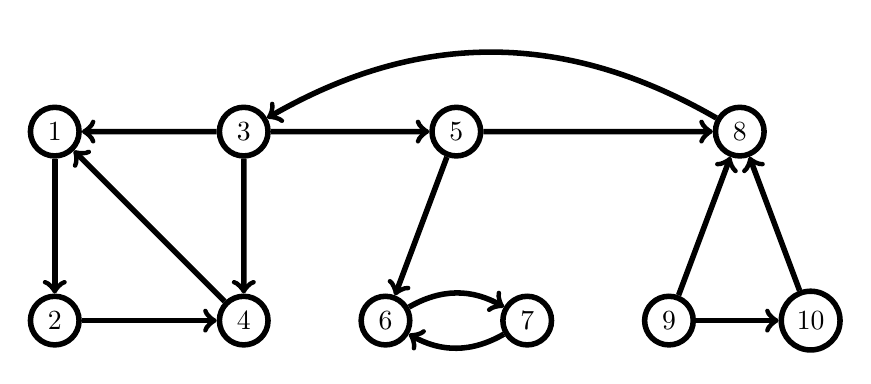
\begin{tikzpicture}[line width=2,scale=1.2]
 \node[circle,draw=black] (1) at (0,2) {$1$};
 \node[circle,draw=black] (2) at (0,0) {$2$};
 \node[circle,draw=black] (3) at (2,2) {$3$};
 \node[circle,draw=black] (4) at (2,0) {$4$};
 \node[circle,draw=black] (5) at (4.25,2) {$5$};
 \node[circle,draw=black] (6) at (3.5,0) {$6$};
 \node[circle,draw=black] (7) at (5,0) {$7$};
 \node[circle,draw=black] (8) at (7.25,2) {$8$};
 \node[circle,draw=black] (9) at (6.5,0) {$9$};
 \node[circle,draw=black] (10) at (8,0) {$10$};
		
 \draw[->] (1) edge (2);
 \draw[->] (2) edge (4);
 \draw[->] (3) edge (1) (3) edge (4) (3) edge (5);
 \draw[->] (4) edge (1);
 \draw[->] (5) edge (6) (5) edge (8); 
 \draw[->] (6) to[bend left] (7);
 \draw[->] (7) to[bend left] (6);
 \draw[->] (8) to[bend right] (3);
 \draw[->] (9) edge (8) (9) edge (10);
 \draw[->] (10) edge (8); 
\end{tikzpicture}
\hfill\,

\noindent Wir wählen als Startknoten den Knoten~$3$ und treffen ansonsten jede Wahl aufsteigend in der Reihenfolge der Knotenindizes.
Die ersten sechs Zeitschritte sind durch die folgende Sequenz von gefärbten Digraphen gegeben, wobei die Knotenfarbe dem aktuellen Farbattribut entspricht und die bereits sondierten Kanten rot markiert sind. Weiterhin geben wir die Rekursionsaufrufe und die Zeitstempel an:

\condclearpage 

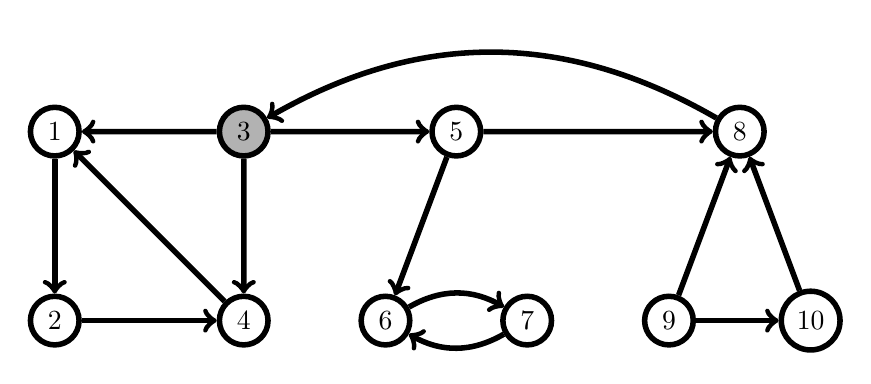
\begin{tikzpicture}[line width=2,scale=1.2]
 \tikzset{gnode/.style ={fill=black!30!,circle,draw}}
 \tikzset{snode/.style ={white,fill=black,circle,draw}}

 \node[circle,draw=black] (1) at (0,2) {$1$};
 \node[circle,draw=black] (2) at (0,0) {$2$};
 \node[gnode] (3) at (2,2) {$3$};
 \node[circle,draw=black] (4) at (2,0) {$4$};
 \node[circle,draw=black] (5) at (4.25,2) {$5$};
 \node[circle,draw=black] (6) at (3.5,0) {$6$};
 \node[circle,draw=black] (7) at (5,0) {$7$};
 \node[circle,draw=black] (8) at (7.25,2) {$8$};
 \node[circle,draw=black] (9) at (6.5,0) {$9$};
 \node[circle,draw=black] (10) at (8,0) {$10$};
		
 \draw[->] (1) edge (2);
 \draw[->] (2) edge (4);
 \draw[->] (3) edge (1) (3) edge (4) (3) edge (5);
 \draw[->] (4) edge (1);
 \draw[->] (5) edge (6) (5) edge (8); 
 \draw[->] (6) to[bend left] (7);
 \draw[->] (7) to[bend left] (6);
 \draw[->] (8) to[bend right] (3);
 \draw[->] (9) edge (8) (9) edge (10);
 \draw[->] (10) edge (8); 
\end{tikzpicture}
\\ $\cc{Tiefensuche}(3)$ 
\\ $\cc{Grau}[3] = 1$

\condclearpage 

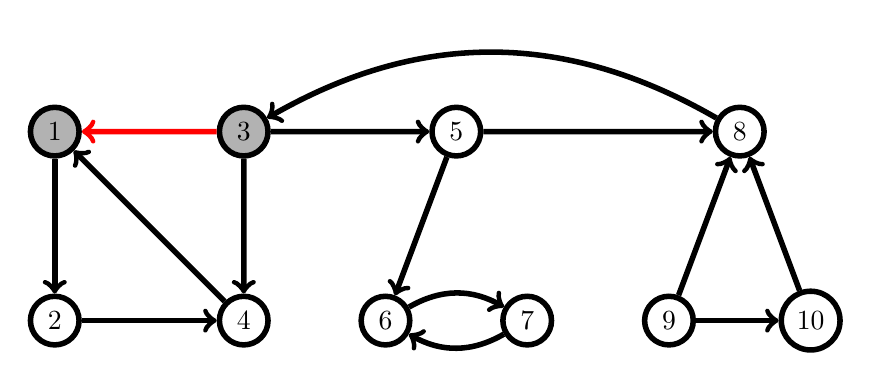
\begin{tikzpicture}[line width=2,scale=1.2]
 \tikzset{gnode/.style ={fill=black!30!,circle,draw}}
 \tikzset{snode/.style ={white,fill=black,circle,draw}}

 \node[gnode] (1) at (0,2) {$1$};
 \node[circle,draw=black] (2) at (0,0) {$2$};
 \node[gnode] (3) at (2,2) {$3$};
 \node[circle,draw=black] (4) at (2,0) {$4$};
 \node[circle,draw=black] (5) at (4.25,2) {$5$};
 \node[circle,draw=black] (6) at (3.5,0) {$6$};
 \node[circle,draw=black] (7) at (5,0) {$7$};
 \node[circle,draw=black] (8) at (7.25,2) {$8$};
 \node[circle,draw=black] (9) at (6.5,0) {$9$};
 \node[circle,draw=black] (10) at (8,0) {$10$};
		
 \draw[->] (1) edge (2);
 \draw[->] (2) edge (4);
 \draw[->,red] (3) edge (1);
 \draw[->] (3) edge (4) (3) edge (5);
 \draw[->] (4) edge (1);
 \draw[->] (5) edge (6) (5) edge (8); 
 \draw[->] (6) to[bend left] (7);
 \draw[->] (7) to[bend left] (6);
 \draw[->] (8) to[bend right] (3);
 \draw[->] (9) edge (8) (9) edge (10);
 \draw[->] (10) edge (8); 
\end{tikzpicture}
\\ $\cc{Tiefensuche}(3) \to \cc{Tiefensuche}(1)$ 
\\ $\cc{Grau}[1] = 2$

\condclearpage 
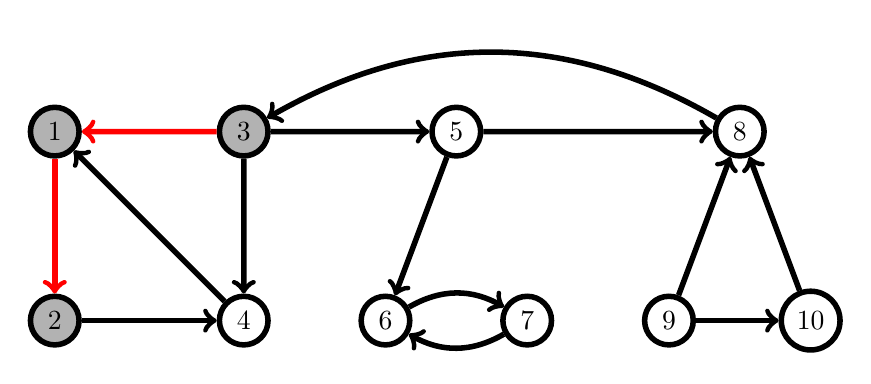
\begin{tikzpicture}[line width=2,scale=1.2]
 \tikzset{gnode/.style ={fill=black!30!,circle,draw}}
 \tikzset{snode/.style ={white,fill=black,circle,draw}}

 \node[gnode] (1) at (0,2) {$1$};
 \node[gnode] (2) at (0,0) {$2$};
 \node[gnode] (3) at (2,2) {$3$};
 \node[circle,draw=black] (4) at (2,0) {$4$};
 \node[circle,draw=black] (5) at (4.25,2) {$5$};
 \node[circle,draw=black] (6) at (3.5,0) {$6$};
 \node[circle,draw=black] (7) at (5,0) {$7$};
 \node[circle,draw=black] (8) at (7.25,2) {$8$};
 \node[circle,draw=black] (9) at (6.5,0) {$9$};
 \node[circle,draw=black] (10) at (8,0) {$10$};
		
 \draw[->,red] (1) edge (2);
 \draw[->] (2) edge (4);
 \draw[->,red] (3) edge (1);
 \draw[->] (3) edge (4) (3) edge (5);
 \draw[->] (4) edge (1);
 \draw[->] (5) edge (6) (5) edge (8); 
 \draw[->] (6) to[bend left] (7);
 \draw[->] (7) to[bend left] (6);
 \draw[->] (8) to[bend right] (3);
 \draw[->] (9) edge (8) (9) edge (10);
 \draw[->] (10) edge (8); 
\end{tikzpicture}
\\ $\cc{Tiefensuche}(3) \to \cc{Tiefensuche}(1) \to \cc{Tiefensuche}(2)$ 
\\ $\cc{Grau}[2] = 3$

\condclearpage 
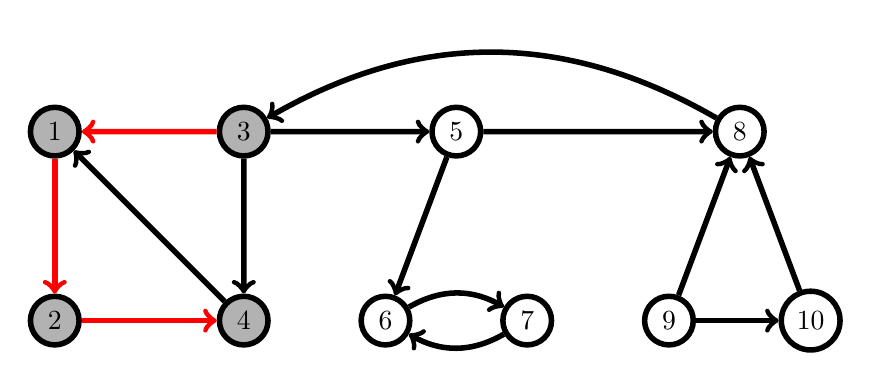
\begin{tikzpicture}[line width=2,scale=1.2]
 \tikzset{gnode/.style ={fill=black!30!,circle,draw}}
 \tikzset{snode/.style ={white,fill=black,circle,draw}}

 \node[gnode] (1) at (0,2) {$1$};
 \node[gnode] (2) at (0,0) {$2$};
 \node[gnode] (3) at (2,2) {$3$};
 \node[gnode] (4) at (2,0) {$4$};
 \node[circle,draw=black] (5) at (4.25,2) {$5$};
 \node[circle,draw=black] (6) at (3.5,0) {$6$};
 \node[circle,draw=black] (7) at (5,0) {$7$};
 \node[circle,draw=black] (8) at (7.25,2) {$8$};
 \node[circle,draw=black] (9) at (6.5,0) {$9$};
 \node[circle,draw=black] (10) at (8,0) {$10$};
		
 \draw[->,red] (1) edge (2);
 \draw[->,red] (2) edge (4);
 \draw[->,red] (3) edge (1);
 \draw[->] (3) edge (4) (3) edge (5);
 \draw[->] (4) edge (1);
 \draw[->] (5) edge (6) (5) edge (8); 
 \draw[->] (6) to[bend left] (7);
 \draw[->] (7) to[bend left] (6);
 \draw[->] (8) to[bend right] (3);
 \draw[->] (9) edge (8) (9) edge (10);
 \draw[->] (10) edge (8); 
\end{tikzpicture}
\\ $\cc{Tiefensuche}(3) \to \cc{Tiefensuche}(1) \to \cc{Tiefensuche}(2) \to \cc{Tiefensuche}(4)$ 
\\ $\cc{Grau}[4] = 4$

\condclearpage

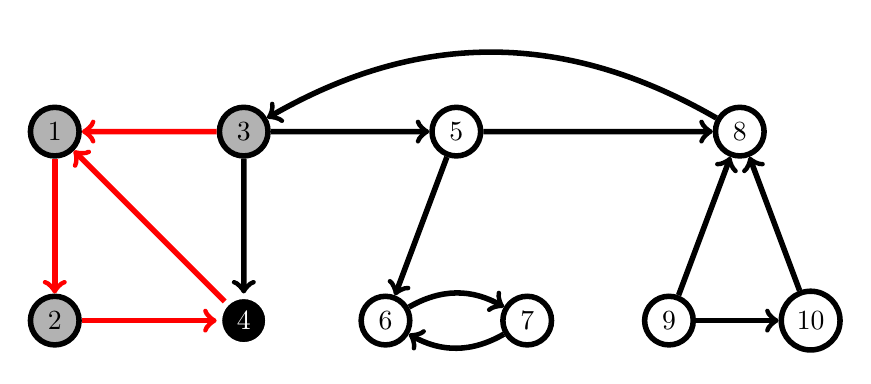
\begin{tikzpicture}[line width=2,scale=1.2]
 \tikzset{gnode/.style ={fill=black!30!,circle,draw}}
\tikzset{snode/.style ={white,fill=black,circle,draw}}

 \node[gnode] (1) at (0,2) {$1$};
 \node[gnode] (2) at (0,0) {$2$};
 \node[gnode] (3) at (2,2) {$3$};
 \node[snode] (4) at (2,0) {$4$};
 \node[circle,draw=black] (5) at (4.25,2) {$5$};
 \node[circle,draw=black] (6) at (3.5,0) {$6$};
 \node[circle,draw=black] (7) at (5,0) {$7$};
 \node[circle,draw=black] (8) at (7.25,2) {$8$};
 \node[circle,draw=black] (9) at (6.5,0) {$9$};
 \node[circle,draw=black] (10) at (8,0) {$10$};
		
 \draw[->,red] (1) edge (2);
 \draw[->,red] (2) edge (4);
 \draw[->,red] (3) edge (1);
 \draw[->] (3) edge (4) (3) edge (5);
 \draw[->,red] (4) edge (1);
 \draw[->] (5) edge (6) (5) edge (8); 
 \draw[->] (6) to[bend left] (7);
 \draw[->] (7) to[bend left] (6);
 \draw[->] (8) to[bend right] (3);
 \draw[->] (9) edge (8) (9) edge (10);
 \draw[->] (10) edge (8); 
\end{tikzpicture}
\\ $\cc{Tiefensuche}(3) \to \cc{Tiefensuche}(1) \to \cc{Tiefensuche}(2)$ 
\\ $\cc{Schwarz}[4] = 5$

\condclearpage 

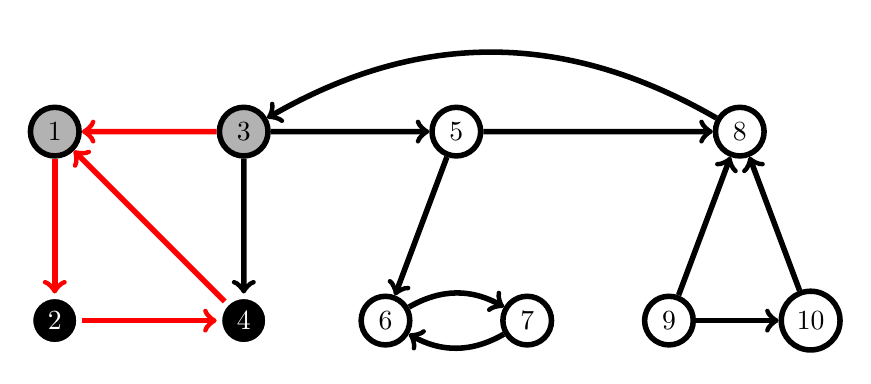
\begin{tikzpicture}[line width=2,scale=1.2]
 \tikzset{gnode/.style ={fill=black!30!,circle,draw}}
 \tikzset{snode/.style ={white,fill=black,circle,draw}}

 \node[gnode] (1) at (0,2) {$1$};
 \node[snode] (2) at (0,0) {$2$};
 \node[gnode] (3) at (2,2) {$3$};
 \node[snode] (4) at (2,0) {$4$};
 \node[circle,draw=black] (5) at (4.25,2) {$5$};
 \node[circle,draw=black] (6) at (3.5,0) {$6$};
 \node[circle,draw=black] (7) at (5,0) {$7$};
 \node[circle,draw=black] (8) at (7.25,2) {$8$};
 \node[circle,draw=black] (9) at (6.5,0) {$9$};
 \node[circle,draw=black] (10) at (8,0) {$10$};
		
 \draw[->,red] (1) edge (2);
 \draw[->,red] (2) edge (4);
 \draw[->,red] (3) edge (1);
 \draw[->] (3) edge (4) (3) edge (5);
 \draw[->,red] (4) edge (1);
 \draw[->] (5) edge (6) (5) edge (8); 
 \draw[->] (6) to[bend left] (7);
 \draw[->] (7) to[bend left] (6);
 \draw[->] (8) to[bend right] (3);
 \draw[->] (9) edge (8) (9) edge (10);
 \draw[->] (10) edge (8); 
\end{tikzpicture}
\\ $\cc{Tiefensuche}(3) \to \cc{Tiefensuche}(1)$ 
\\ $\cc{Schwarz}[2] = 6$

\condclearpage 

\noindent Wir steigen zum Zeitpunkt $\cc{Schwarz}[8]=14$ mit der Illustration wieder ein:

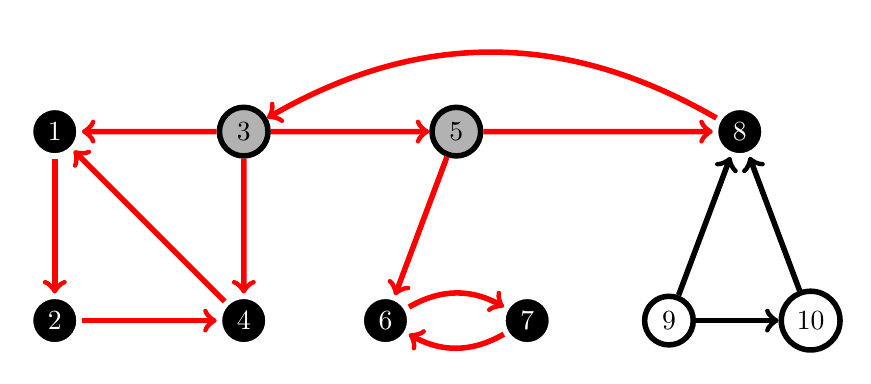
\begin{tikzpicture}[line width=2,scale=1.2]
 \tikzset{gnode/.style ={fill=black!30!,circle,draw}}
 \tikzset{snode/.style ={white,fill=black,circle,draw}}

 \node[snode] (1) at (0,2) {$1$};
 \node[snode] (2) at (0,0) {$2$};
 \node[gnode] (3) at (2,2) {$3$};
 \node[snode] (4) at (2,0) {$4$};
 \node[gnode] (5) at (4.25,2) {$5$};
 \node[snode] (6) at (3.5,0) {$6$};
 \node[snode] (7) at (5,0) {$7$};
 \node[snode] (8) at (7.25,2) {$8$};
 \node[circle,draw=black] (9) at (6.5,0) {$9$};
 \node[circle,draw=black] (10) at (8,0) {$10$};
		
 \draw[->,red] (1) edge (2);
 \draw[->,red] (2) edge (4);
 \draw[->,red] (3) edge (1);
 \draw[->,red] (3) edge (4) (3) edge (5);
 \draw[->,red] (4) edge (1);
 \draw[->,red] (5) edge (6) (5) edge (8); 
 \draw[->,red] (6) to[bend left] (7);
 \draw[->,red] (7) to[bend left] (6);
 \draw[->,red] (8) to[bend right] (3);
 \draw[->] (9) edge (8) (9) edge (10);
 \draw[->] (10) edge (8); 
\end{tikzpicture}
\\ $\cc{Tiefensuche}(3) \to \cc{Tiefensuche}(5)$ 
\\ $\cc{Schwarz}[8] = 14$

\condclearpage 

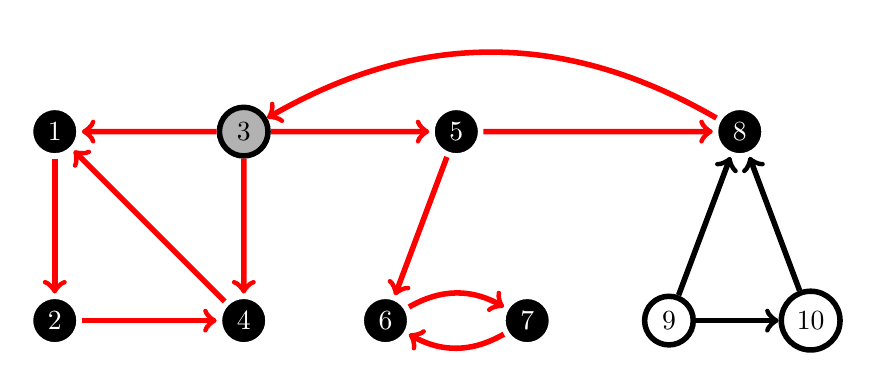
\begin{tikzpicture}[line width=2,scale=1.2]
 \tikzset{gnode/.style ={fill=black!30!,circle,draw}}
 \tikzset{snode/.style ={white,fill=black,circle,draw}}

 \node[snode] (1) at (0,2) {$1$};
 \node[snode] (2) at (0,0) {$2$};
 \node[gnode] (3) at (2,2) {$3$};
 \node[snode] (4) at (2,0) {$4$};
 \node[snode] (5) at (4.25,2) {$5$};
 \node[snode] (6) at (3.5,0) {$6$};
 \node[snode] (7) at (5,0) {$7$};
 \node[snode] (8) at (7.25,2) {$8$};
 \node[circle,draw=black] (9) at (6.5,0) {$9$};
 \node[circle,draw=black] (10) at (8,0) {$10$};
		
 \draw[->,red] (1) edge (2);
 \draw[->,red] (2) edge (4);
 \draw[->,red] (3) edge (1);
 \draw[->,red] (3) edge (4) (3) edge (5);
 \draw[->,red] (4) edge (1);
 \draw[->,red] (5) edge (6) (5) edge (8); 
 \draw[->,red] (6) to[bend left] (7);
 \draw[->,red] (7) to[bend left] (6);
 \draw[->,red] (8) to[bend right] (3);
 \draw[->] (9) edge (8) (9) edge (10);
 \draw[->] (10) edge (8); 
\end{tikzpicture}
\\ $\cc{Tiefensuche}(3)$ 
\\ $\cc{Schwarz}[5] = 15$

\condclearpage 

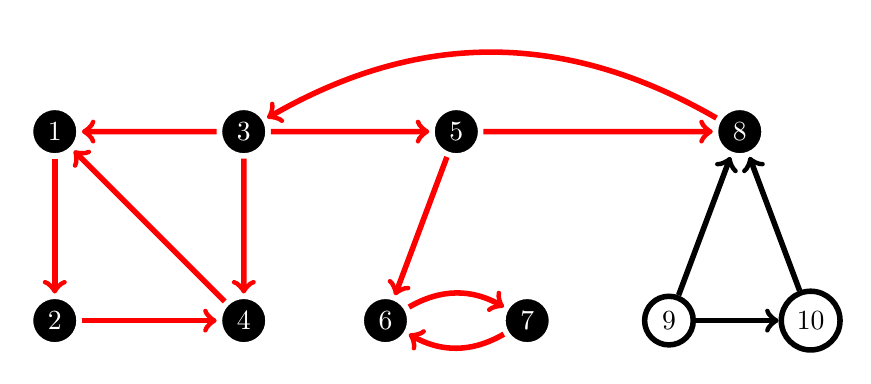
\begin{tikzpicture}[line width=2,scale=1.2]
 \tikzset{gnode/.style ={fill=black!30!,circle,draw}}
 \tikzset{snode/.style ={white,fill=black,circle,draw}}

 \node[snode] (1) at (0,2) {$1$};
 \node[snode] (2) at (0,0) {$2$};
 \node[snode] (3) at (2,2) {$3$};
 \node[snode] (4) at (2,0) {$4$};
 \node[snode] (5) at (4.25,2) {$5$};
 \node[snode] (6) at (3.5,0) {$6$};
 \node[snode] (7) at (5,0) {$7$};
 \node[snode] (8) at (7.25,2) {$8$};
 \node[circle,draw=black] (9) at (6.5,0) {$9$};
 \node[circle,draw=black] (10) at (8,0) {$10$};
		
 \draw[->,red] (1) edge (2);
 \draw[->,red] (2) edge (4);
 \draw[->,red] (3) edge (1);
 \draw[->,red] (3) edge (4) (3) edge (5);
 \draw[->,red] (4) edge (1);
 \draw[->,red] (5) edge (6) (5) edge (8); 
 \draw[->,red] (6) to[bend left] (7);
 \draw[->,red] (7) to[bend left] (6);
 \draw[->,red] (8) to[bend right] (3);
 \draw[->] (9) edge (8) (9) edge (10);
 \draw[->] (10) edge (8); 
\end{tikzpicture}
\\ $\cc{Schwarz}[3] = 16$

\noindent Nun muss ein neuer Knoten gewählt werden (Knoten $9$) um die vollständige Tiefensuche für den ganzen Digraphen zu beenden:

\condclearpage 
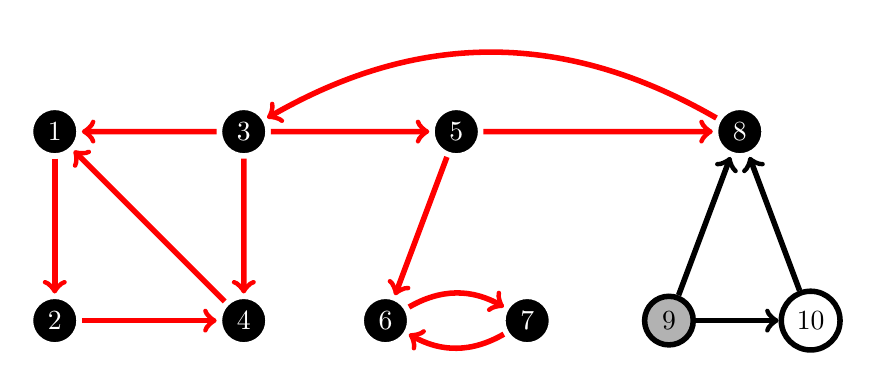
\begin{tikzpicture}[line width=2,scale=1.2]
 \tikzset{gnode/.style ={fill=black!30!,circle,draw}}
 \tikzset{snode/.style ={white,fill=black,circle,draw}}

 \node[snode] (1) at (0,2) {$1$};
 \node[snode] (2) at (0,0) {$2$};
 \node[snode] (3) at (2,2) {$3$};
 \node[snode] (4) at (2,0) {$4$};
 \node[snode] (5) at (4.25,2) {$5$};
 \node[snode] (6) at (3.5,0) {$6$};
 \node[snode] (7) at (5,0) {$7$};
 \node[snode] (8) at (7.25,2) {$8$};
 \node[gnode] (9) at (6.5,0) {$9$};
 \node[circle,draw=black] (10) at (8,0) {$10$};
		
 \draw[->,red] (1) edge (2);
 \draw[->,red] (2) edge (4);
 \draw[->,red] (3) edge (1);
 \draw[->,red] (3) edge (4) (3) edge (5);
 \draw[->,red] (4) edge (1);
 \draw[->,red] (5) edge (6) (5) edge (8); 
 \draw[->,red] (6) to[bend left] (7);
 \draw[->,red] (7) to[bend left] (6);
 \draw[->,red] (8) to[bend right] (3);
 \draw[->] (9) edge (8) (9) edge (10);
 \draw[->] (10) edge (8); 
\end{tikzpicture}
\\ $\cc{Tiefensuche}(9)$ 
\\ $\cc{Grau}[9] = 17$

\condclearpage 
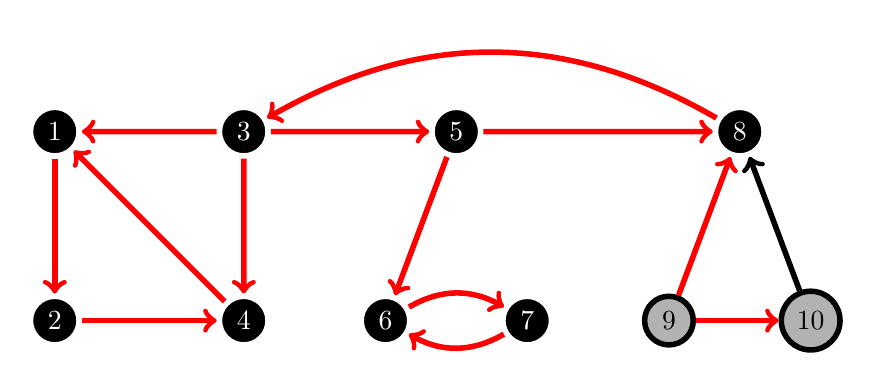
\begin{tikzpicture}[line width=2,scale=1.2]
 \tikzset{gnode/.style ={fill=black!30!,circle,draw}}
 \tikzset{snode/.style ={white,fill=black,circle,draw}}

 \node[snode] (1) at (0,2) {$1$};
 \node[snode] (2) at (0,0) {$2$};
 \node[snode] (3) at (2,2) {$3$};
 \node[snode] (4) at (2,0) {$4$};
 \node[snode] (5) at (4.25,2) {$5$};
 \node[snode] (6) at (3.5,0) {$6$};
 \node[snode] (7) at (5,0) {$7$};
 \node[snode] (8) at (7.25,2) {$8$};
 \node[gnode] (9) at (6.5,0) {$9$};
 \node[gnode] (10) at (8,0) {$10$};
		
 \draw[->,red] (1) edge (2);
 \draw[->,red] (2) edge (4);
 \draw[->,red] (3) edge (1);
 \draw[->,red] (3) edge (4) (3) edge (5);
 \draw[->,red] (4) edge (1);
 \draw[->,red] (5) edge (6) (5) edge (8); 
 \draw[->,red] (6) to[bend left] (7);
 \draw[->,red] (7) to[bend left] (6);
 \draw[->,red] (8) to[bend right] (3);
 \draw[->,red] (9) edge (8) (9) edge (10);
 \draw[->] (10) edge (8); 
\end{tikzpicture}
\\ $\cc{Tiefensuche}(9) \to \cc{Tiefensuche}(10)$ 
\\ $\cc{Grau}[10] = 18$

\condclearpage 
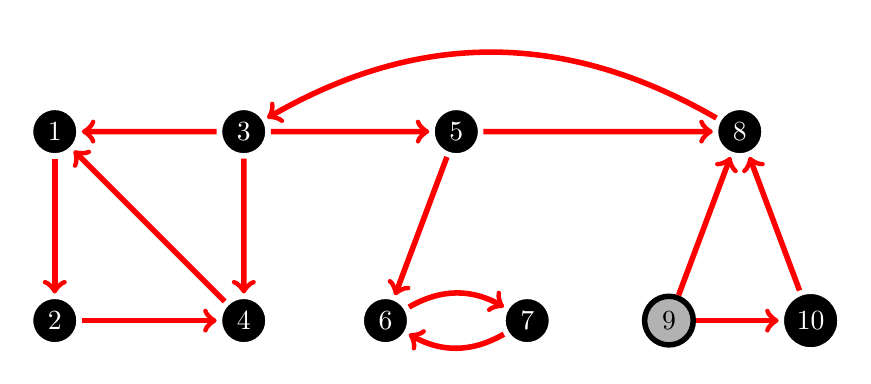
\begin{tikzpicture}[line width=2,scale=1.2]
 \tikzset{gnode/.style ={fill=black!30!,circle,draw}}
 \tikzset{snode/.style ={white,fill=black,circle,draw}}

 \node[snode] (1) at (0,2) {$1$};
 \node[snode] (2) at (0,0) {$2$};
 \node[snode] (3) at (2,2) {$3$};
 \node[snode] (4) at (2,0) {$4$};
 \node[snode] (5) at (4.25,2) {$5$};
 \node[snode] (6) at (3.5,0) {$6$};
 \node[snode] (7) at (5,0) {$7$};
 \node[snode] (8) at (7.25,2) {$8$};
 \node[gnode] (9) at (6.5,0) {$9$};
 \node[snode] (10) at (8,0) {$10$};
		
 \draw[->,red] (1) edge (2);
 \draw[->,red] (2) edge (4);
 \draw[->,red] (3) edge (1);
 \draw[->,red] (3) edge (4) (3) edge (5);
 \draw[->,red] (4) edge (1);
 \draw[->,red] (5) edge (6) (5) edge (8); 
 \draw[->,red] (6) to[bend left] (7);
 \draw[->,red] (7) to[bend left] (6);
 \draw[->,red] (8) to[bend right] (3);
 \draw[->,red] (9) edge (8) (9) edge (10);
 \draw[->,red] (10) edge (8); 
\end{tikzpicture}
\\ $\cc{Tiefensuche}(9)$ 
\\ $\cc{Schwarz}[10] = 19$

\condclearpage 
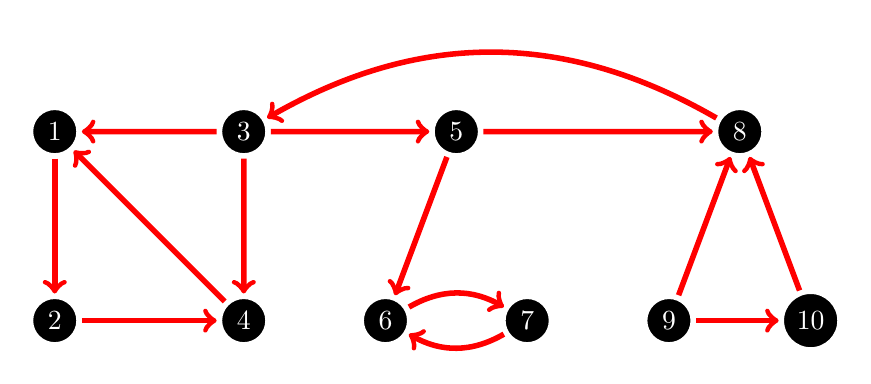
\begin{tikzpicture}[line width=2,scale=1.2]
 \tikzset{gnode/.style ={fill=black!30!,circle,draw}}
 \tikzset{snode/.style ={white,fill=black,circle,draw}}

 \node[snode] (1) at (0,2) {$1$};
 \node[snode] (2) at (0,0) {$2$};
 \node[snode] (3) at (2,2) {$3$};
 \node[snode] (4) at (2,0) {$4$};
 \node[snode] (5) at (4.25,2) {$5$};
 \node[snode] (6) at (3.5,0) {$6$};
 \node[snode] (7) at (5,0) {$7$};
 \node[snode] (8) at (7.25,2) {$8$};
 \node[snode] (9) at (6.5,0) {$9$};
 \node[snode] (10) at (8,0) {$10$};
		
 \draw[->,red] (1) edge (2);
 \draw[->,red] (2) edge (4);
 \draw[->,red] (3) edge (1);
 \draw[->,red] (3) edge (4) (3) edge (5);
 \draw[->,red] (4) edge (1);
 \draw[->,red] (5) edge (6) (5) edge (8); 
 \draw[->,red] (6) to[bend left] (7);
 \draw[->,red] (7) to[bend left] (6);
 \draw[->,red] (8) to[bend right] (3);
 \draw[->,red] (9) edge (8) (9) edge (10);
 \draw[->,red] (10) edge (8); 
\end{tikzpicture}
\\ $\cc{Schwarz}[9] = 20$

\noindent Nun sind alle Knoten schwarz gefärbt und die Tiefensuche ist beendet.
\end{bsp}

%Als Beispiel kann man die TS mit dem Startknoten $1$ im Fall von $N$:
%\[
%	\begin{array}{llll}
%	1: & 2, & 4 
%	\\ 2: & 3
%	\\ 3: & 
%	\\ 4: & 2, & 3, & 5
%	\\ 5: & 6
%	\\ 6: & 4
%	\\ 7: & 6
%	\end{array}
%\]
%betrachten. Wir protokollieren die Änderungen wann welche TSen aufgerufen und beendet werden und wie sich die Farben der Knoten ändern. *****

\begin{bem}
	Bevor wir die Eigenschaften der Tiefensuche diskutieren, analysieren wir ihre Laufzeit.
\end{bem} 

\begin{thm}
\label{thm:laufzeit-tiefensuche}
Es sei ein Digraph $D=(V,A)$ durch eine Adjazenzliste gegeben. Sei weiterhin $u \in V$ ein Knoten. Dann hat die Laufzeit von $\cc{Tiefensuche}(u)$ die Ordnung $O(|V|+|A|)$ und die Laufzeit von $\cc{Vollständige-Tiefensuche}(D)$ die Ordnung $\Theta(|V|+|A|)$.
\end{thm}

\begin{proof}
Die Initialisierung hat offenbar die Laufzeit $\Theta(|V|)$.
Der Aufwand für die $\cc{TS}$ (= Tiefensuche) setzt sich aus den folgenden Operationen zusammen, die man den Knoten und Kanten zuordnet: 
%
\begin{equation*}
	\cc{weiss} 
	\ \xrightarrow{\cc{TS}(u)\text{ Start}} \ 
	\cc{grau}
	\ \xrightarrow{\text{Sondierung von }N[u]}
	\ \cc{schwarz} 
	\  \xrightarrow{\cc{TS}(u)\text{ Ende}} \ 
\end{equation*} 

%Hier wird $TS$ als Abkürzung für $\cc{Tiefensuche}$ benutzt.
\noindent Für die (vollständige) Tiefensuche ist der Aufwand somit höchstens $O(|V|+|A|)$, denn der Aufwand pro Knoten ist $O(1)$, da kein Knoten $u$ wegen der Änderung der Farben mehr als ein Mal untersucht werden kann. Genauso ist der Aufwand pro Kante stets $O(1)$, da eine Kante $(u,v)$ genau dann sondiert wird, wenn man $u$ entdeckt, der Knoten $u$ wird aber höchstens ein Mal entdeckt.

Weiterhin ist klar, dass der Aufwand bei der vollständigen Tiefensuche $\Omega(|V|+|A|)$ ist, da die for-Schleife in der vollständigen Tiefensuche dafür sorgt, dass jeder Knoten (und damit auch jede Kante) entdeckt wird. 
\end{proof}


%\begin{thm}
%	Sei $G=(V,E)$ Digraph mit $m \in \N$ Kanten und $n \in \N$ Knoten, der durch eine Adjazenzliste gegeben ist. Sei $s \in V$. Dan gilt für die Tiefensuche auf $G$ mit dem Startknoten $s$:
%	\begin{enumerate}[(a)]
%		\item Die Laufzeit des Verfahrens ist $O(m+n)$ (das heißt, höchstens $c(m+n)$ für eine Konstante $c>0$).
%		\item Die Menge aller Knoten von $G$, die von $s$ aus durch einen Pfad erreichbar sind ist genau die Menge der Knoten, die während der Ausführung entdeckt werden. 
%		\item Der Graph $G$ enthält genau dann einen von $s$ aus erreichbaren Zyklus, wenn während der Ausführung beim Sondieren einer der Kanten $(u,v)$ die Farbe von $v$ grau ist. 
%	\end{enumerate} 
%\end{thm}
%\begin{proof}
%	(a): Während der Ausführung werden die folgende Operationen ausgeführt: Änderung der Farben und Aufruf der TS für unterschiedliche Knoten sowie Sondierung der Kanten. Jeder entdeckte Knoten ändert seine Farbe von weiß zu grau und anschließend zu schwarz. Da eine TS nur für einen weißen Knoten gestartet wird, wird die TS für jeden Knoten höchstens ein mal ausgeführt. Somit dauert die Bearbeitung von jedem Knoten (Farbenänderung, Aufruf der TS) $O(1)$ Zeiteinheiten. Eine Kante $(u,v)$ wird genau dann sondiert, wenn die TS für $u$ aufgerufen wird. Somit kann jede Kante höchstens ein mal sondiert werden. Das Sondieren jeder Kante beträgt dadurch höchstens $O(1)$ Zeiteinheiten. Der Gesamtaufwand der TS mit dem Startknoten $s$ ist somit $O(m+n)$. 
%	
%	(b): Seien $u_1,\ldots,u_k$ alle Knoten, die während der Ausführung entdeckt werden und seien $u_1,\ldots,u_k$ in dieser Reihenfolge entdeckt ($u_1$ ist der erste entdeckte Knoten, $u_2$ der zweite usw.). Dann ist $u_1$ von $s$ aus erreichbar, denn $u_1=s$. Die TS für einen Knoten $u_j$ mit $j > 1$ wird aus einer TS für einen Knoten $u_i$ aufgerufen, der im Moment der Aufuruf von $TS(u_j)$ bereits entdeckt ist. Man hat also $j< i$. Wenn $u_j$ von $s$ aus erreichbar ist, so ist auch $u_i$ von $s$ aus erreichbar, da $(u_i,u_j)$ eine Kante von $G$ ist. Somit folgt durch Induktion über $j$, das jeder Knoten $u_j$ von $s$ aus erreichbar ist. 
%	
%	Umgekehrt zeigen wir nun, dass jeder Knoten $v \in V$, der von $s$ aus erreichbar ist, während der Ausführung entdeckt wird. Sei $(v_0,\ldots,v_k)$ ein Pfad von $s$ nach $v$. Wir zeigen nun, dass jeder Knoten $v_j$ dieses Pfades entdeckt wird. Für $v_0=s$ gilt die Aussage offensichtlich. Wird ein Knoten $v_j$ mit $j < k$ entdeckt, so entdeckt man den Knoten $v_{j+1}$ spätestens beim Sondieren der Kante $(v_j,v_{j+1})$ innerhalb der TS für $v_j$. Es kann als durch Induktion über $j$ gezeigt werden, dass alle $v_j$ und insbesondere auch $v_k=v$ entdeckt werden.
%	
%	(c): Der Beweis von (c) ist analog zum Beweis von (b) und wird hier nicht angeführt. (Aufgabe)
%\end{proof}
%

\begin{defn} 
Ähnlich wie bei Breitensuche erzeugt die Vorgängerabbildung $\pi$ den sogenannten \textbf{Vor\-gänger\-teil\-graphen} eines Digraphen $D=(V,A)$, der formal durch $D_\pi=(V,A_\pi)$ mit
\[
A_\pi = \left\{(\pi[v],v) : v \in V \text{ und } \pi[v] \neq \cc{nil}\right\}
\]
definiert ist.
Für jede Tiefensuche ist der Vorgängerteilgraph zu jedem Zeitpunkt ein Wald.

Nach dem Abschluss der vollständigen Tiefensuche wird $D_\pi$ daher als \textbf{Tiefensuchwald} bezeichnet, der aus einem oder mehreren \textbf{Tiefensuchbäumen} zusammengesetzt ist.
\end{defn} 

\begin{bsp} 
In Beispiel~\ref{bsp:tiefensuche} ist die Vorgängerabbildung nach abgeschlossener vollständiger Tiefensuche beginnend mit dem Knoten $3$ durch $\pi=[3,1,\cc{nil},2,3,5,6,5,\cc{nil},9]$ gegeben.
Der zugehörige Tiefensuchwald ist also

\begin{center} 
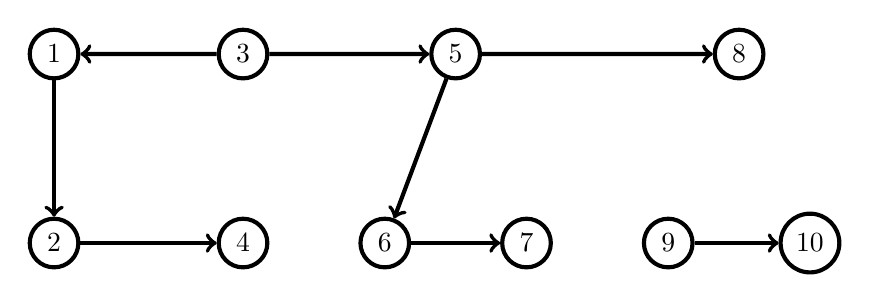
\begin{tikzpicture}[line width=1.5,scale=1.2]
 \node[circle,draw=black] (1) at (0,2) {$1$};
 \node[circle,draw=black] (2) at (0,0) {$2$};
 \node[circle,draw=black] (3) at (2,2) {$3$};
 \node[circle,draw=black] (4) at (2,0) {$4$};
 \node[circle,draw=black] (5) at (4.25,2) {$5$};
 \node[circle,draw=black] (6) at (3.5,0) {$6$};
 \node[circle,draw=black] (7) at (5,0) {$7$};
 \node[circle,draw=black] (8) at (7.25,2) {$8$};
 \node[circle,draw=black] (9) at (6.5,0) {$9$};
 \node[circle,draw=black] (10) at (8,0) {$10$};
		
 \draw[->] (1) edge (2);
 \draw[->] (2) edge (4);
 \draw[->] (3) edge (1) (3) edge (5);
 \draw[->] (5) edge (6) (5) edge (8); 
 \draw[->] (6) edge (7);
 \draw[->] (9) edge (10);
\end{tikzpicture}
\end{center}

\noindent\underline{Achtung:} Der Tiefensuchwald hängt davon ab, mit welchem Knoten die Tiefensuche beginnt und in welcher Reihenfolge die Entscheidungen im Algorithmus getrofffen werden.
\end{bsp} 

\begin{lem}
	Sei $D= (V,A)$ ein Digraph. 
	Nach der Initialisierung der Tiefensuche und während der Ausführung der vollständigen Tiefensuche ist der Vorgängerteilgraph $D_\pi$ stets ein gerichteter Wald. Die Wurzeln der Bäume dieses Waldes sind genau die Knoten $u \in V$, für welche $\cc{TS}(u)$ aus der Hauptschleife der vollständigen Tiefensuche aufgerufen wurde. 
\end{lem} 
\begin{proof} 
Wir führen wieder Induktion nach der Anzahl der Färbungen von Knoten mit der Farbe Grau.
%	Die Anzahl der Knoten, die während der Ausführung entdeckt werden nimmt während der Ausführung zu.
Nach der Initialisierung und am Anfang der ersten Ausführung auf dem Startknoten $s \in V$ ist $D_\pi$ der leere Graph (es wurde noch kein Vorgänger gesetzt) auf der Knotenmenge~$V$, und für diesen gilt die Behauptung.
%Die Behauptung gilt also am Anfang der Ausführung.  Am Anfang ist kein Knoten grau gefärbt und kein Vorgänger gesetzt, sodass $D_\pi$ ein Wald ohne Kanten ist.

Beachten Sie, dass ein noch weißer Knoten weder Wurzel noch Knoten mit Vorgänger in einem der aktuellen Tiefensuchbäume sein kann.
Wird ein Knoten $v$ gerade grau gefärbt, so wurde er über eine Kante $(u,v) \in A$ entdeckt.
Der Startknoten $u$ dieser Kante gehört vor der Grau-Färbung von~$v$ zu einem Tiefensuchbaum, der nach Hinzunahme der Kante $(u,v)$ weiterhin ein gerichteter Baum ist.
Da~$v$ vor seiner Entdeckung zu keinem Tiefensuchbaum gehörte, wird du die Hinzunahme der Kante $(u,v)$ in $D_\pi$ kein Zyklus geschlossen und somit bleibt $D_\pi$ weiterhin ein gerichteter Wald.
\end{proof} 


%\begin{bem}
%		Wir bezeichnen die Tiefensuche kurz als $\cc{TS}$, die vollständige Tiefensuche als $\cc{VTS}$ und die Intialisierung der Tiefensuche als $\cc{TSI}$. 
%\end{bem} 

\condclearpage
\subsection{Eigenschaften der Tiefensuche}


\begin{lem} \label{ts:key:lemma} 
	Sei $D=(V,A)$ ein Digraph und sei $s \in V$. Wir betrachten die Ausführung von $\cc{TS}(s)$ nach einer Initialisierung der Tiefensuche für $D$. Während der Ausführung sind nach jeder Knotenfärbung die folgenden Aussagen erfüllt:
	\begin{enuma} 
		\item Die Menge der grauen Knoten bildet einen gerichteten Weg $(u_0,\ldots,u_m)$ in $D_\pi$, der im Knoten $u_0=s$ beginnt. 
		\item Der Kontrollfluss befindet sich im Aufruf von $\cc{TS}(u_m)$. 
		\item Für jedes $i=1,\ldots,m$, wurde $\cc{TS}(u_i)$  aus $\cc{TS}(u_{i-1})$ aufgerufen und die Aufrufe $\cc{TS}(u_1),\ldots,\cc{TS}(u_m)$ sind noch nicht zu Ende ausgeführt. 
	\end{enuma} 
	Darüber hinaus gilt: ein Knoten $v$ wird während der Ausführung von $\cc{TS}(s)$ genau dann entdeckt, wenn in~$D$ ein $(s,v)$-Pfad existiert. 
\end{lem} 
\begin{proof}
	Für die Behauptungen (a)--(c) benutzen wir vollständige Induktion über die Anzahl der Färbungen während der Ausführung von $\cc{TS}(s)$. Die erste Färbung ist die Grau-Färbung von~$s$. In diesem Moment der Ausführung gelten die Behauptungen für den Weg der Länge $0$, der aus dem Knoten $s$ besteht. Angenommen, die Behauptungen gelten nach $k \in\N$ Färbungen. Wir betrachten den Pfad $(u_0,\ldots,u_m)$, für den die Behauptungen gelten.
	
	Wird während der Ausführung von $\cc{TS}(u_m)$, ein weißer Knoten $v$ entdeckt, so wird $\cc{TS}(v)$ aufgerufen, in der $v$ grau gefärbt wird, sodass nach $k+1$ Färbungen die Behauptungen für den Pfad $(u_0,\ldots,u_m,v)$ erfüllt sind. 
	
	Sind während der Ausführung von $\cc{TS}(u_m)$ alle von~$u_m$ ausgehende Kanten sondiert, so wird~$u_m$ schwarz gefärbt, die Ausführung von $\cc{TS}(u_m)$ terminiert und der Kontrollfluss kehrt zum Aufruf $\cc{TS}(u_{m-1})$ zurück. In diesem Fall gelten die Behauptungen nach $k+1$ Färbungen für den Pfad $(u_0,\ldots,u_{m-1})$. 
	
\condclearpage

	Nun zeigen wir die letzte Behauptung: wenn ein Knoten $v$ entdeckt wird, dann bilden laut der Behauptung (a) die Knoten, die im Moment der Entdeckung von $v$ grau sind, einen $(s,v)$-Pfad. Umgekehrt, sei $v \in V$ ein Knoten, für den ein $(s,v)$-Pfad $(v_0,\ldots,v_t)$ in $D$ existiert. Wir zeigen, dass der Knoten $v$ entdeckt wird. Angenommen, das wäre falsch. Wir zeigen durch Induktion über $i=0,1,\ldots,t$, dass der Knoten $v_i$ entdeckt wird. Der Knoten $v_0=s$ wird entdeckt. Sei also $1 \le i < t$ und nehmen wir an, dass $v_0,\ldots,v_{i-1}$ entdeckt werden. Da $v_{i-1}$ entdeckt wird, wird die Kante $(v_{i-1},v_i)$ sondiert, sodass $v_i$ spätestens beim Sondieren der Kante $(v_{i-1},v_i)$ entdeckt wird (eventuell wird~$v_i$ bereits früher von einem anderen Knoten aus entdeckt). 
\end{proof} 

\begin{kor}[Theorem der weißen Pfade]\label{kor:weisse:pfade} 
	Sei $D=(V,A)$ ein Digraph und sei $u \in V$.
	Sind die Farbattribute der Knoten von $V$ auf weiß/grau/schwarz gesetzt, und ist $u$ ein weißer Knoten, für den man $\cc{TS}(u)$ startet, so wird ein weißer Knoten $v \in V$ während der Ausführung von $\cc{TS}(u)$ genau dann entdeckt, wenn vor der Ausführung von $\cc{TS}(u)$ ein $(u,v)$-Pfad in~$D$ existiert, der nur aus weißen Knoten besteht. 
\end{kor} 
\begin{proof}
	Bei der Ausführung von $\cc{TS}(u)$ wird die Tiefensuche für Knoten, die vor der Ausführung grau oder schwarz waren, nicht aufgerufen. Somit entspricht die Ausführung von $\cc{TS}(u)$ einer Ausführung der Tiefensuche auf dem Teilgraphen von~$D$, der durch die Knoten induziert ist, die vor der Ausführung weiß waren.
	
	Die Behauptung folgt damit aus der letzten Behauptung von Lemma~\ref{ts:key:lemma}. 
\end{proof} 


\begin{thm} \label{thm:ts:und:zyklen} 
	Sei $D=(V,A)$ ein Digraph und sei $s \in V$. Wir betrachten die Ausführung von $\cc{TS}(s)$ nach einer Initialisierung der Tiefensuche für $D$. Der Digraph $D$ enthält genau dann einen von $s$ aus erreichbaren Zyklus, wenn während der Ausführung beim Sondieren einer Kante $(u,v)$ die Farbe von $v$ grau ist. 
\end{thm}
\begin{proof}	
	Sei zunächst während der Ausführung beim Sondieren einer Kante $(u,v)$ die Farbe von~$v$ grau. Nach Lemma~\ref{ts:key:lemma} bildet die Menge der Knoten, die grau gefärbt sind, einen $(s,u)$-Weg $(u_0,\ldots,u_m)$ mit $u_0=s$ und $u=u_m$. Der Knoten $v$ ist also ein Knoten $u_j$ auf diesem Weg. Somit ist $(u_j,\ldots,u_m,u_j)$ ein Zyklus in $D$.
	
\condclearpage

	Umgekehrt, sei $Z$ ein Zyklus, der von $s$ aus durch einen Pfad erreichbar ist. Wir zeigen, dass während der Ausführung eine Kante von~$Z$ sondiert wird, deren Endknoten grau ist. Sei $u$ der Knoten im Zyklus $Z$, der während der Ausführung von $\cc{TS}(s)$ unter allen Knoten von $Z$ als erster entdeckt wird. Nach der Grau-Färbung von $u$ existiert nach Lemma~\ref{ts:key:lemma} ein $(s,u)$-Pfad $(u_0,\ldots,u_m)$ mit $s=u_0$ und $u_m=u$, der keinen anderen Knoten von $Z$ außer $u$ enthält. Wir schreiben $Z$ als $(v_0,\ldots,v_t,v_0)$ mit $v_0=u$.
	
\condclearpage
	
	Unmittelbar vor der Entdeckung von~$u$ ist $v_0,\ldots,v_t$ ein Pfad aus weißen Knoten. Nach Korollar~\ref{kor:weisse:pfade} wird während der Ausführung von $\cc{TS}(u)$ der Knoten $v_t$ entdeckt.
	
	Wir wenden nun Lemma~\ref{ts:key:lemma} auf den Teilgraphen von~$D$ an, der durch die Knoten induziert wird, die unmittelbar vor der Entdeckung von $u$ weiß sind. Da $(v_0,\ldots,v_t)$ ein Pfad in diesem Teilgraphen ist, wird $v_t$ während der Ausführung von $\cc{TS}(u)$ entdeckt. Bei der Entdeckung von~$v_t$ gibt es zwei Arten von grauen Knoten:
\begin{itemize}
 \item Die Knoten, welche vor dem Aufruf von $\cc{TS}(u)$ grau gefärbt wurden, sind $u_0,\ldots,u_m$.
 \item Die Knoten, die während der Ausführung von $\cc{TS}(u)$ und bis zum Aufruf von $\cc{TS}(v_t)$ grau gefärbt wurden, bilden einen $(u,v_t)$-Weg.
\end{itemize}

\condclearpage

\noindent Es folgt, dass nach der Entdeckung von $v_t$ der Weg aus grauen Knoten mit dem Knoten $u_0=s$ beginnt und die Form $(u_0,\ldots,u_m, w_1,\ldots,w_\ell)$ mit $w_\ell =v_t$ hat. Beim Sondieren der Kante $(v_t,u)$ ist also die Farbe von $u=u_m$ grau. 
\end{proof}

\begin{bem}
Nach Theorem~\ref{thm:ts:und:zyklen} kann daher die Tiefensuche benutzt werden, um zu entscheiden, ob ein gegebener Digraph $D$ einen Zyklus enthält, bzw. ob ein gegebener ungerichteter Graph $G$ einen Kreis enthält.
\end{bem}


\begin{bem}
Eine wichtige Eigenschaft der Tiefensuche ist der Zusammenhang von Entdeckungszeit und Abarbeitungszeit eines Knotens. Es stellt sich heraus, dass diese Zeitpunkte im folgenden Sinne eine Klammerstruktur aufweisen:

Stellen wir die Entdeckungszeit eines Knotens $u$ durch den Ausdruck \glqq $(u$\grqq\ und die Abarbeitungszeit von $u$ durch den Ausdruck \glqq $u)$\grqq\ dar, dann ergibt die gesamte Historie, über alle Knoten des (Di)Graphen hinweg gesehen, einen korrekt geklammerten Ausdruck.
\end{bem}

\begin{bsp} 
%	Die Relation der Lebenszeit Intervallen zu einander kann durch geklammerte Ausdrücke dargestellt werden. 
	Zur Illustration dieses Zusammenhangs sehen wir uns wieder Beispiel~\ref{bsp:tiefensuche} an.

\hfill
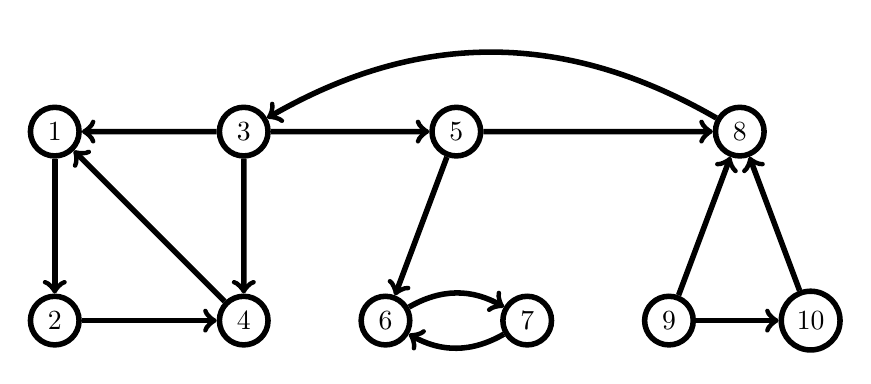
\begin{tikzpicture}[line width=2,scale=1.2]
 \node[circle,draw=black] (1) at (0,2) {$1$};
 \node[circle,draw=black] (2) at (0,0) {$2$};
 \node[circle,draw=black] (3) at (2,2) {$3$};
 \node[circle,draw=black] (4) at (2,0) {$4$};
 \node[circle,draw=black] (5) at (4.25,2) {$5$};
 \node[circle,draw=black] (6) at (3.5,0) {$6$};
 \node[circle,draw=black] (7) at (5,0) {$7$};
 \node[circle,draw=black] (8) at (7.25,2) {$8$};
 \node[circle,draw=black] (9) at (6.5,0) {$9$};
 \node[circle,draw=black] (10) at (8,0) {$10$};
		
 \draw[->] (1) edge (2);
 \draw[->] (2) edge (4);
 \draw[->] (3) edge (1) (3) edge (4) (3) edge (5);
 \draw[->] (4) edge (1);
 \draw[->] (5) edge (6) (5) edge (8); 
 \draw[->] (6) to[bend left] (7);
 \draw[->] (7) to[bend left] (6);
 \draw[->] (8) to[bend right] (3);
 \draw[->] (9) edge (8) (9) edge (10);
 \draw[->] (10) edge (8); 
\end{tikzpicture}
\hfill\,

	\noindent Die Daten der Zeitstempel der Tiefensuche sind in folgender Tabelle zusammengefasst:
	\begin{table}[H]
		\centering
		\begin{tabular}{|c|c|c|c|c|c|c|c|c|c|c|}
			\hline
			\textbf{Knoten $u$}        & \textbf{1} & \textbf{2} & \textbf{3} & \textbf{4} & \textbf{5} & \textbf{6} & \textbf{7} & \textbf{8} & \textbf{9} & \textbf{10} \\ \hline
			\textbf{$\cc{Grau}[u]$}    & 2          & 3          & 1          & 4          & 8          & 9          & 10         & 13         & 17         & 18          \\ \hline
			\textbf{$\cc{Schwarz}[u]$} & 7          & 6          & 16         & 5          & 15         & 12         & 11         & 14         & 20         & 19          \\ \hline
		\end{tabular}
	\end{table}
	\noindent Nach obiger Vorschrift erhalten wir damit den zugehörigen Klammerausdruck
	\[
	(3\ (1\ (2\ (4\ 4)\ 2)\ 1)\ (5\ (6\ (7\ 7)\ 6)\ (8\ 8)\ 5)\ 3)\ (9\ (10\ 10)\ 9)
	\]
\end{bsp} 

\begin{bem} 	
Eine andere Möglichkeit diese Klammerstruktur auszudrücken benötigt das Konzept der Lebenszeitintervalle:
\end{bem}

\begin{defn}
	Bzgl. einer vollständigen Tiefensuche auf einem Digraphen $D=(V,A)$ mit Startknoten $s \in V$ definieren wir das \textbf{Lebenszeitintervall} eines Knotens $u \in V$ als die Menge
	\[
			I_u:=\setcond{t \in \Z}{ \cc{Grau}[u] \le t \le \cc{Schwarz}[u]}. 
	\]
\end{defn} 

\begin{thm}[Klammerungstheorem]
\label{thm:klammerung}
Bei der vollständigen Tiefensuche auf einem Digraphen $D=(V,A)$ ist für jedes Paar von Knoten $u$ und $v$ genau eine der drei folgenden Bedingungen erfüllt:
\begin{enuma}

 \item $I_u \cap I_v = \emptyset$  und weder $u$ noch $v$ ist im Tiefensuchwald ein Nachfahre des anderen.

 \item $I_u \subseteq I_v$ und $u$ ist im Tiefensuchwald ein Nachfahre von $v$.

 \item $I_v \subseteq I_u$ und $v$ ist im Tiefensuchwald ein Nachfahre von $u$.

\end{enuma}
\end{thm}
\begin{proof}
	Die Aussage ist symmetrisch bzgl. $u$ und $v$. Wir  nehmen also ohne Beschränkung der Allgemeinheit an, dass während der Ausführung der vollständigen Tiefensuche der Knoten~$u$ vor dem Knoten~$v$ entdeckt wurde. Ist die Tiefensuche für $v$ nach der Terminierung der Tiefensuche für $u$ aufgerufen worden, so gilt $I_u \cap I_v = \emptyset$ und die Knoten~$u$ und~$v$ liegen in verschiedenen Bäumen des Tiefensuchwaldes.
	
	Ansonsten ist die Tiefensuche für $v$ vor der Terminierung der Tiefensuche für $u$ aufgerufen worden. Das bedeutet, dass der Knoten $v$ während der Ausführung von $u$ entdeckt worden ist. Der Aufruf von $\cc{TS}(v)$ erfolgt also durch eine Folge von rekursiven Aufrufen 
	\[
		\cc{TS}(u) \xrightarrow{} \ldots \xrightarrow{} \cc{TS}(v) .
	\] 
	Somit terminiert $\cc{TS}(v)$ vor $\cc{TS}(u)$. Es gilt also $I_v \subseteq I_u$ und $v$ ist Nachfahre von $u$. 
\end{proof}



\begin{bem}
Als direkte Konsequenz des Klammerungstheorems erhalten wir eine Charakterisierung der Nachfahren im Tiefensuchwald eines gegebenen Knotens.
\end{bem} 

\begin{kor}
\label{cor:nachfahre-tiefenwald}
Der Knoten $v$ ist in einem Tiefensuchwald eines Digraphen genau dann ein echter Nachfahre eines Knotens $u$, wenn
\[
\cc{Grau}[u] < \cc{Grau}[v] < \cc{Schwarz}[v]  < \cc{Schwarz}[u].
\]
\end{kor}

\begin{bem} 
Eine alternative Charakterisierung der Nachfahreneigenschaft in Tiefensuchwäldern, die allerdings über die Farben der Knoten während der Suche geht, wird uns später bei den Anwendungen der Tiefensuche nützlich sein. 
\end{bem}


\begin{defn}
\label{def:kantenarten-tiefensuche}
Die Kanten $(u,v) \in A$ die bei einer Tiefensuche auf $D=(V,A)$ sondiert werden, werden in Abhängigkeit davon, welche Farbe $v$ beim Sondieren von $(u,v)$ hat und in welchem Zusammenhang $\cc{Grau}[u]$  und $\cc{Grau}[v]$ stehen, in die folgenden Arten unterteilt: 
\begin{center} 
\begin{tabular}{l|l}
	Art von $(u,v) \in A$ & Bedingung beim Sondieren 
	\\ \hline 
	\textbf{Baumkante} & $\cc{Farbe}[v]=\cc{weiss}$ 
\\	\textbf{Rückwärtskante} & $\cc{Farbe}[v] = \cc{grau}$
\\ \textbf{Vorwärtskante} & $\cc{Farbe}[v] = \cc{schwarz}$, $\cc{Grau}[u] < \cc{Grau}[v]$
\\ \textbf{Querkante} & $\cc{Farbe}[v] = \cc{schwarz}$, $\cc{Grau}[u] > \cc{Grau}[v]$
\end{tabular} 
\end{center} 
Die Baumkanten sind genau die Kanten des Tiefensuchwaldes $D_\pi$. 
\end{defn}

\begin{bsp} Im Fall der Adjazenzliste 
	\begin{align*}
		 1: & \ [2,4] 
		 \\ 2: & \  [3,4]
		 \\ 3: & \ [1]
		 \\  4: & \ [3]
	\end{align*}
 wird  während der Ausführung von $\cc{Tiefensuche}(1)$ die folgende Unterteilung der Kanten in die vier Arten festgelegt: 
	\begin{center} 
	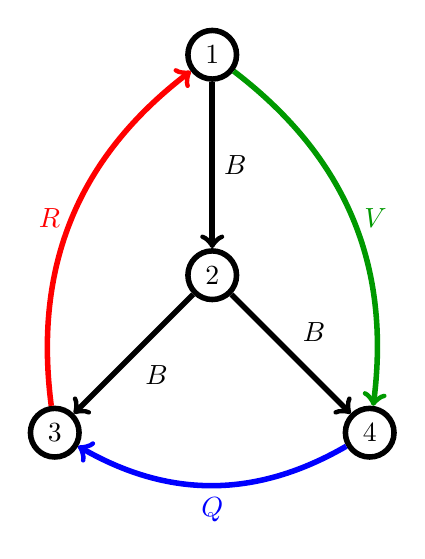
\begin{tikzpicture}[line width=2,scale=2]
		\node[circle,draw=black] (1) at (0,3.4) {$1$};
		\node[circle,draw=black] (2) at (0,2) {$2$};
		\node[circle,draw=black] (3) at (-1,1) {$3$};
		\node[circle,draw=black] (4) at (1,1) {$4$};
		\draw[->] (1) edge node[right]{$B$}(2) (2) edge node[below right]{$B$} (3) (2) edge node[above right]{$B$} (4);
		\draw[->,red] (3) edge[bend left] node[left]{$R$} (1);
		\draw[->,green!60!black]  (1) edge[bend left] node[right]{$V$} (4);
		\draw[->,blue] (4) edge[bend left] node[below]{$Q$} (3);
	\end{tikzpicture} 
	\end{center} 
\end{bsp} 

\begin{bem} 
	Wird die Unterteilung der Kanten in die vier Arten Baum-, Rückwärts- Vorwärts- und Querkante im Rahmen der vollständigen Tiefensuche durchgeführt, so ist jede Kante, welche zwei Bäume des Tiefensuchwaldes verbindet eine Querkante.
	
	Eine Querkante $(u,v)$ kann auch zwei Knoten des gleichen Tiefensuchbaumes
verbinden, solange $u$ nicht Vorfahre von $v$ ist.
\end{bem} 


%\begin{remark}
%Durch die TS können die Kanten $(u,v)$ des Graphen in drei Arten klassifiziert werden: die Vorwärtskanten (beim sondieren von $(u,v)$ ist $v$ weiß), die Rückwärtskarten (beim sondieren der Kante ist $v$ grau) und die Querkanten (beim Sondieren der Kante ist $v$ schwarz). Die Menge aller  $\{u,v\}$ derart, dass $(u,v) \in E$ als ein Vorwärtskante klassifiziert wurde, ist Kantenmenge eines Baums. Die Knotenmenge dieses Baums ist die Menge aller entdeckten Knoten.
%\end{remark}

\begin{bsp} 
Wir schauen uns wiederum die Tiefensuche aus Beispiel~\ref{bsp:tiefensuche} an und, basierend auf den bereits erhobenen Daten, stellen wir die Klassifikation der Kanten des bearbeiteten Digraphen farbkodiert in folgender Abbildung dar.
Dabei sind Baumkanten schwarz, Rückwärtskanten rot, Vorwärtskanten blau und Querkanten grün markiert.

\begin{center} 
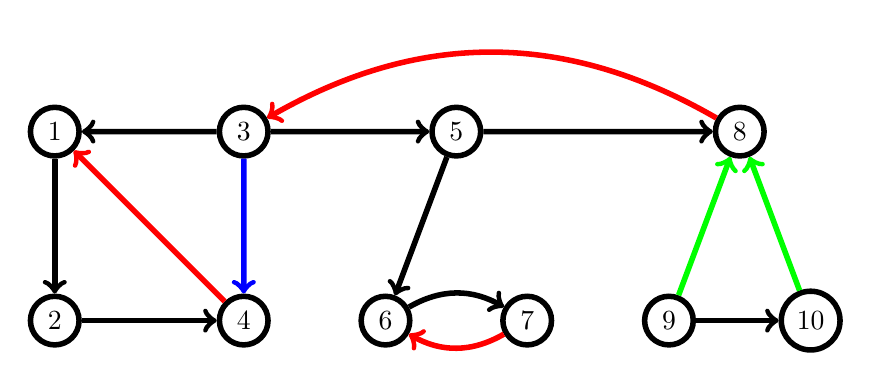
\begin{tikzpicture}[line width=2,scale=1.2]
 \node[circle,draw=black] (1) at (0,2) {$1$};
 \node[circle,draw=black] (2) at (0,0) {$2$};
 \node[circle,draw=black] (3) at (2,2) {$3$};
 \node[circle,draw=black] (4) at (2,0) {$4$};
 \node[circle,draw=black] (5) at (4.25,2) {$5$};
 \node[circle,draw=black] (6) at (3.5,0) {$6$};
 \node[circle,draw=black] (7) at (5,0) {$7$};
 \node[circle,draw=black] (8) at (7.25,2) {$8$};
 \node[circle,draw=black] (9) at (6.5,0) {$9$};
 \node[circle,draw=black] (10) at (8,0) {$10$};

% Baumkanten
 \draw[->] (1) edge (2);
 \draw[->] (2) edge (4);
 \draw[->] (3) edge (1) (3) edge (5);
 \draw[->] (5) edge (6) (5) edge (8); 
 \draw[->] (6) to[bend left] (7);
 \draw[->] (9) edge (10);

% Rückwärtskanten
 \draw[->,red] (4) edge (1);
 \draw[->,red] (7) to[bend left] (6);
 \draw[->,red] (8) to[bend right] (3);

% Vorwärtskanten
 \draw[->,blue] (3) edge (4);
	
% Querkanten
 \draw[->,green] (9) edge (8);
 \draw[->,green] (10) edge (8); 
	
\end{tikzpicture}
\end{center} 
\end{bsp} 


\begin{bem}
In einem ungerichteten Graphen können bei der Klassifizierung der Kanten nach Definition~\ref{def:kantenarten-tiefensuche} Mehrdeutigkeiten auftreten, da die Kanten $uv$ und $vu$ übereinstimmen.
Daher klassifizieren wir hier die Kanten in Abhängigkeit davon, ob der Algorithmus zuerst $uv$ oder zuerst $vu$ sondiert.

Als Besonderheit bei ungerichteten Graphen bobachten wir, dass während einer
Tiefensuche weder Vorwärts- noch Querkanten auftreten:
\end{bem}

\begin{thm}
Bei einer Tiefensuche auf einem ungerichteten Graphen $G$ ist jede Kante entweder eine Baumkante oder eine Rückwärtskante.
\end{thm}

\begin{proof}
Sei $(u,v)$ eine beliebige Kante von~$G$ und seien die Knoten~$u$ und~$v$ so bezeichnet, dass $\cc{Grau}[u] < \cc{Grau}[v]$ gilt.
Die Tiefensuche muss daher den Knoten~$v$ entdeckt und fertig abgearbeitet haben, bevor~$u$ fertig abgearbeitet ist.
In der Zwischenzeit ist der Knoten~$u$ stets grau.

Falls die Durchmusterung die Kante zuerst in der Richtung von~$u$ nach~$v$ sondiert, so ist~$v$ bis dahin unentdeckt (also weiß) gewesen, da die Kante sonst bereits in Gegenrichtung sondiert worden wäre.
Mit anderen Worten, die Kante $(u,v)$ ist eine Baumkante.

Falls die Durchmusterung die Kante zuerst in der Richtung von~$v$ nach~$u$ sondiert, so ist die Kante $(u,v)$ eine Rückwärtskante, da~$u$ zu dem Zeitpunkt der Sondierung noch grau ist.
\end{proof}


\begin{bem}
	Analog zur Breitensuche kann man eine Tiefensuche auch ohne Rekursion umsetzen.
	Dies hat praktische Vorteile, weil der Programmstack nicht  belastet wird.
	Dazu ersetzt man die Warteschlange $Q$ durch einen sogenannten \textbf{Stack} ($=$ \textbf{Stapel}).
%	Für die Tiefensuche kann ein Stack auf der Basis von einem Array umgesetzt werden. 
\end{bem}

\begin{defn} 
Ein \textbf{Stack}~$S$ ist eine Liste $S=[s_1,\ldots,s_k]$, die mit drei Grundoperationen ausgestattet ist:
\begin{itemize}
 \item $\cc{Top}(S)$: Das \textbf{oberste} Element~$s_1$ von~$S$ wird zurückgegeben, aber nicht aus $S$ entfernt.

 \item $\cc{Pop}(S)$: Das \textbf{oberste} Element~$s_1$ von~$S$ wird zurückgegeben und aus $S$ entfernt.
 Nach der Operation gilt $S=[s_2,\ldots,s_k]$.

 \item $\cc{Push}(S,u)$: Das Element~$u$ wird am \textbf{Anfang} ($=$ oben) von~$S$ hinzugefügt.
 Nach Ausführung dieser Operation gilt also $S=[u,s_1,\ldots,s_k]$. 
\end{itemize}
\end{defn} 

\begin{bem}
Erinnern Sie sich, dass Warteschlangen nach dem FIFO-Prinzip (First In - First Out) arbeiten.
Analog arbeiten Stacks nach dem LIFO-Prinzip (Last In - First Out)

Genau wie Warteschlangen können Stacks mit höchstens $n \in \N$ Elementen auf der Basis von Arrays der Länge~$n$ umgesetzt werden, sodass die Laufzeit der Grundoperationen $\Theta(1)$ Zeiteinheiten beträgt. 
\end{bem} 
	
\begin{bem}
Konvertieren wir nun die rekursive Tiefensuche in einen nicht-rekursiven Algorithmus:

%Als $\cc{Top}(S)$ bezeichnen wir das oberste Element des Stacks. Durch $\cc{Pop}(S)$ erfolgt die Entfernung und Rückgabe des obersten Elements. Durch $\cc{Push}(S,u)$ wird ein neues Element $u$ auf den Stack gelegt.
Für einen Knoten $u$ indizieren wir die Elemente in $N[u]$ mit den Zahlen $0$ bis $\deg(u)-1$, wobei $\deg(u)$ der Grad des Knotens $u$ ist. Wir führen ein Array $\cc{ind}$ ein, in dem durch $\cc{ind}[u]$ notiert wird, dass beim Sondieren der Nachbarn von $u \in V$ der Knoten $v=N[u][\cc{ind}[u]]$ als  nächster dran ist. Ist $\cc{ind}[u]= \deg(u)$, so hat man alle Nachbarn von $u$ sondiert. Wir setzen am Anfang $\cc{ind}[u]=0$ für alle $u \in V$, färben den Startknoten $s$ grau und legen $s$ auf $S$. Auf diese Weise lassen sich mit Hilfe von $S$ und $\cc{ind}$ die gerade laufenden rekursiven Aufrufe der Tiefensuche simulieren: 

	\begin{algorithm}[H]
		\caption{$\cc{Tiefensuche-mit-Stack}(s)$} 
		\begin{algorithmic}[1]
			\STATE Stack $S$ für höchstens $|V|$ Elemente anlegen
			\STATE $\cc{Farbe}[s] = \cc{grau}$ 
			\STATE $\cc{push}(S,s)$
			\STATE Liste $\cc{Ind}$  mit $\cc{Ind}[u]=0$ für alle $u \in V$ anlegen
			\WHILE{$S$ nicht leer }
			\STATE $u:= \cc{top}(S)$ \quad \COMMENT{Suche für $u$ läuft weiter}
			\IF{$\cc{ind}[u] = \deg(u)$} 
			\STATE $\cc{pop}(S)$   \quad \COMMENT{Suche für $u$ wird beendet}
			\STATE $\cc{Farbe}[u] := \cc{schwarz}$
			\ELSE
			\STATE $v=N[u][\cc{ind}[u]]$ \quad \COMMENT{Sondierung der Nachbarn von $u$ wird fortgesetzt} 
			\STATE $\cc{ind}[u]:=\cc{ind}[u]+1$				
			\IF{$\cc{Farbe}[v] = \cc{weiss}$}
			\STATE $\cc{Farbe}[v] = \cc{grau}$ \quad \COMMENT{Neuer Knoten ist entdeckt}
			\STATE $\cc{push}(S,v)$ \quad \COMMENT{Suche für $v$ wird gestartet}
			\ENDIF 
			\ENDIF 
			\ENDWHILE  
		\end{algorithmic}
	\end{algorithm}

	Die weiteren Daten (Vorgängerabbildung und Zeitstempel), die man im Rahmen der rekursiven Tiefensuche berechnet, kann man auch in der obigen iterativen Version an den entsprechenden Stellen berechnen. 
\end{bem}

\begin{bem}\ Umsetzung: 
\lstinputlisting{Code/dfs.sage}
\end{bem} 


\condclearpage
\subsection{Anwendung I -- Topologisches Sortieren}

\begin{defn} 
Sei $D=(V,A)$ ein Digraph mit $n$ Knoten.
Eine \textbf{topologische Sortierung} von $D$ ist eine Anordnung $v_1,\ldots,v_n$ seiner Knoten, so dass für jede Kante $(v_i,v_j) \in A$ die Bedingung $i < j$ gilt.
Das heißt, der Startknoten einer jeden Kante kommt in der Anordnung vor dem Endknoten.
\end{defn} 

\begin{bem}
Man kann eine topologische Sortierung auch als horizontale Anordnung der Knoten von~$D$ auffassen, so dass jede Kante von links nach rechts zeigt.

Sehen wir uns den folgenden Digraphen an, der Zusammenhänge zwischen verschiedenen Graphenbegriffen darstellt:

\vspace{1em}
\hfill
\begin{tikzpicture}[]
 \node[ellipse,draw=black] (1) at (0,3) {Teilgraph};
 \node[ellipse,draw=black] (2) at (6,3) {Weg};
 \node[ellipse,draw=black] (3) at (12,3) {Zyklus};
 \node[ellipse,draw=black] (4) at (0,0) {Digraph};
 \node[ellipse,draw=black] (5) at (6,0) {Graph};
 \node[ellipse,draw=black] (6) at (12,0) {Pfad};
% \node[ellipse,draw=black] (7) at (4,0) {Teilpfad};
		
 \draw[->,line width=0.5mm] (4) edge (5); 
 \draw[->,line width=0.5mm] (5) edge (1) (5) edge (2) (5) edge (3) (5) edge (6);
 \draw[->,line width=0.5mm] (6) edge (2) (6) edge (3);
\end{tikzpicture}
\hfill\,

\condclearpage

\noindent Eine topologische Sortierung dieses Digraphen ist folgende horizontale Anordnung der Knoten:

\hfill
\begin{tikzpicture}[]
 \node[ellipse,draw=black] (1) at (9,0) {Teilgraph};
 \node[ellipse,draw=black] (2) at (18,0) {Weg};
 \node[ellipse,draw=black] (3) at (22.5,0) {Zyklus};
 \node[ellipse,draw=black] (4) at (0,0) {Digraph};
 \node[ellipse,draw=black] (5) at (4.5,0) {Graph};
 \node[ellipse,draw=black] (6) at (13.5,0) {Pfad};
% \node[ellipse,draw=black] (7) at (10,0) {Teilpfad};

% 4 5 1 6 2 3
		
 \draw[->,line width=0.5mm] (4) edge (5); 
 \draw[->,line width=0.5mm] (5) edge (1) (5) to[bend right] (6);
 \draw[->,line width=0.5mm] (5) to[bend left] (2);
 \draw[->,line width=0.5mm] (5) to[bend right] (3); 
 \draw[->,line width=0.5mm] (6) edge (2) (6) to[bend left] (3);
\end{tikzpicture}
\hfill\,
\end{bem}

\begin{bem}
Diese Veranschaulichung zeigt, dass es nicht möglich ist, einen Digraphen topologisch zu sortieren, wenn er einen Zyklus enthält.
Im Folgenden werden wir sehen, wie man mit einer Tiefensuche jeden \textbf{azyklischen} Digraphen topologisch sortieren kann.
Als Konsequenz ergibt sich:
\end{bem} 

\begin{prop}
Ein Digraph besitzt genau dann eine topologische Sortierung, wenn er azyklisch ist.
\end{prop}

\begin{bem}
Einige Anwendungen des topologischen Sortierens:
\begin{itemize}
 \item \textbf{makefile}: In welcher Reihenfolge sollten einzelne Teilprojekte in einem großen Programmierprojekt kompiliert werden, damit die bestehenden Abhängigkeiten respektiert werden?
% Die Kanten des Digraphen sind durch die Paare target-prerequisite gegeben. Die targets sollen in einer topologisch sortierten Reihenfolge abgearbeitet werden. 
 \item Sequenzieren von Aufträgen (engl.~\textbf{scheduling}).
 \item Eine \textbf{lineare Erweiterung} einer partiellen Ordnung berechnen.
\end{itemize}
\end{bem}


\begin{thm}
	Nach der Ausführung der vollständigen Tiefensuche auf einem azyklischen Digraphen $D=(V,A)$ ist die Anordnung der Knoten $u \in V$ in der absteigenden Reihenfolge nach $\cc{Schwarz}[u]$ eine topologische Sortierung. Diese Anordnung kann während der Tiefensuche in der Zeit $\Theta(|V|+|A|)$ berechnet werden. 
\end{thm}

\begin{proof}
	Wir betrachten eine Kante $(u,v) \in A$. Ist $v$ vor $u$ entdeckt worden, so wird während der Ausführung von $\cc{TS}(v)$ der Knoten $u$ nicht entdeckt, denn sonst gäbe es einen $(v,u)$-Pfad und somit auch einen Zyklus in $D$. Das bedeutet, dass in diesem Fall $\cc{TS}(v)$ vor $\cc{TS}(u)$ terminiert. Es gilt also $\cc{Schwarz}[v] < \cc{Schwarz}[u]$. 
	
	Wird $u$ vor $v$ entdeckt, so wird $v$ während der Ausführung von $\cc{TS}(u)$ spätestens beim Sondieren von $(u,v)$ entdeckt. In diesem Fall terminiert $\cc{TS}(v)$ ebenfalls vor $\cc{TS}(u)$, und es gilt wieder $\cc{Schwarz}[v] < \cc{Schwarz}[u]$.
\end{proof}




\subsection{Anwendung II -- Starke Zusammenhangskomponenten}

\begin{defn}
Sei $D=(V,A)$ ein Digraph. Zwei	Knoten $u,v \in V$ heißen \textbf{gegenseitig erreichbar}, wenn es einen $(u,v)$-Pfad sowie einen $(v,u)$-Pfad in~$D$ gibt. 

Gegenseitige Erreichbarkeit ist eine Äquivalenzrelation auf $V$. Die Äquivalenzklassen bzgl. dieser Relation nennt man \textbf{starke Zusammenhangskomponenten} (SZK) von $D$. 
\end{defn} 

\begin{bsp}
Im folgenden Beispiel (gerichteter Gittergraph) sind die starken Zusammenhangskomponenten mit mehr als einem Knoten farblich hinterlegt:

\hfill
	\includegraphics[width=0.6\textwidth]{Code/strongly_connected_comp.pdf}
\hfill\,
\end{bsp}


\begin{defn}
	Für einen Digraphen $D = (V,A)$ führen wir den sogenannten
 \textbf{transponierten Graphen} $D^\top = (V,A^\top)$ mit
 \[
 A^\top := \{(u,v) \in V \times V : (v,u) \in A\}
 \]
 ein. 
Wir erhalten also $D^\top$ aus $D$, indem wir die Orientierung aller Kanten von $D$ umdrehen.
\end{defn} 


\begin{prop}
\label{beob:d-vs-dt}
Der zu einem Digraphen $D=(V,A)$ transponierte Graph $D^\top$ hat dieselben starken Zusammenhangskomponenten wie~$D$.
\end{prop}
\begin{proof}
Dies folgt direkt aus folgender Beobachtung: Für zwei Knoten $u,v \in V$, für die ein $(u,v)$-Pfad in $D$ existiert, ist der \glqq Rückweg\grqq\ ein $(v,u)$-Pfad in $D^\top$.
\end{proof}

\begin{bem}  \label{szk:algo}
	Sei $D = (V,A)$ Digraph. Zur Berechnung der SZKn von $D$ kann der folgende Algorithmus benutzt werden, den wir als $\cc{SZK}(D)$ bezeichnen: 
\begin{itemize}
	\item \textbf{Phase~1: Anordnung.} Ordne mit Hilfe der vollständigen Tiefensuche auf $D$ die Knotenmenge $V$ in absteigender Reihenfolge $u_1,\ldots,u_n$ der Abarbeitungszeit ($n:=|V|$). Es reicht dafür beim Abarbeiten eines Knotens, den Knoten zu einer Liste mit $n$ Elementen hinzuzufügen (und die Liste vom Ende beginnend zu füllen). 
	\item \textbf{Phase~2: Berechnung der Komponenten.} Führe eine vollständige Tiefensuche auf $D^\top$ durch, bei der über die Knoten $u \in V$ in der oben bestimmten Reihenfolge $u_1,\ldots,u_n$ iteriert wird. Dabei entdeckt jeder Aufruf der Tiefensuche aus der vollständigen Tiefensuche die Knoten einer starken Zusammenhangskomponente.
\end{itemize} 

\noindent Wie man Phase~2 genau umsetzt hängt unter anderem davon ab, in welchem Format man die SZK speichern möchte. 
\end{bem} 

\begin{bem}
Der Algorithmus im Pseudocode:
\begin{algorithm}[H]
\caption{$\cc{SZK}(D)$}
 \begin{algorithmic}[1]
  \STATE\label{line:szhk0} $\cc{Vollständige-Tiefensuche}(D)$
  \STATE berechne $D^\top$
  \STATE\label{line:szhk1} $\cc{Vollständige-Tiefensuche}(D^\top)$
  \STATE\label{line:szhk2} $\quad$ durchlaufe dabei die Hauptschleife in absteigender Reihenfolge des Arrays $\cc{Schwarz}$ von~$D$
  \STATE gib die Knotenmengen der Bäume im Tiefensuchwald $(D^\top)_\pi$ zurück
 \end{algorithmic}
\end{algorithm}
\end{bem}

\begin{bem} Umsetzung: 
\lstinputlisting{Code/szk.sage}
\end{bem} 

\begin{thm}
	\label{thm:starke-zshgk-laufzeit}
	Ist ein Digraph $D=(V,A)$ als Adjazenzliste gegeben, so hat der Algorithmus $\cc{SZK}(D)$ die Laufzeit $\Theta(|V|+|A|)$.
\end{thm}
\begin{proof}
	Die Berechnung von $D^\top$ sowie die beiden vollständigen Tiefensuchen benötigen jeweils  $\Theta(|V|+|A|)$ Elementaroperationen. 
\end{proof}


\begin{bsp}
	\label{bsp:starke-zusammenhangskomponenten}
	Wir berechnen die SZKn des Digraphen aus Beispiel~\ref{bsp:tiefensuche}:
	
{\centering
\begin{tabular}{m{.05\textwidth}m{.4\textwidth}}
$D$
	&
	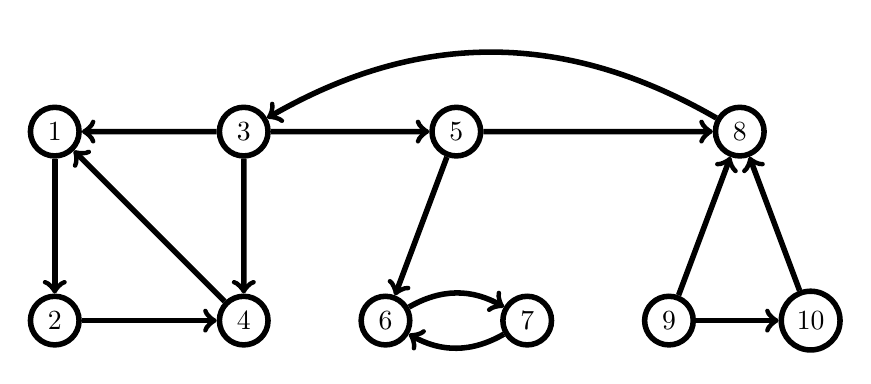
\begin{tikzpicture}[line width=2,scale=1.2]
	 \node[circle,draw=black] (1) at (0,2) {$1$};
	 \node[circle,draw=black] (2) at (0,0) {$2$};
	 \node[circle,draw=black] (3) at (2,2) {$3$};
	 \node[circle,draw=black] (4) at (2,0) {$4$};
	 \node[circle,draw=black] (5) at (4.25,2) {$5$};
	 \node[circle,draw=black] (6) at (3.5,0) {$6$};
	 \node[circle,draw=black] (7) at (5,0) {$7$};
	 \node[circle,draw=black] (8) at (7.25,2) {$8$};
	 \node[circle,draw=black] (9) at (6.5,0) {$9$};
	 \node[circle,draw=black] (10) at (8,0) {$10$};
		
		\draw[->] (1) edge (2);
		\draw[->] (2) edge (4);
		\draw[->] (3) edge (1) (3) edge (4) (3) edge (5);
		\draw[->] (4) edge (1);
		\draw[->] (5) edge (6) (5) edge (8); 
		\draw[->] (6) to[bend left] (7);
		\draw[->] (7) to[bend left] (6);
		\draw[->] (8) to[bend right] (3);
		\draw[->] (9) edge (8) (9) edge (10);
		\draw[->] (10) edge (8); 
	\end{tikzpicture}
\end{tabular}

	\begin{table}[H]
		\centering
		\begin{tabular}{|c|c|c|c|c|c|c|c|c|c|c|}
			\hline
			\textbf{Knoten $u$}        & \textbf{1} & \textbf{2} & \textbf{3} & \textbf{4} & \textbf{5} & \textbf{6} & \textbf{7} & \textbf{8} & \textbf{9} & \textbf{10} \\ \hline
			\textbf{$\cc{Schwarz}[u]$} & 7          & 6          & 16         & 5          & 15         & 12         & 11         & 14         & 20         & 19          \\ \hline
		\end{tabular}
	\end{table}

\begin{tabular}{m{.05\textwidth}m{.4\textwidth}m{.05\textwidth}m{.4\textwidth}}
$D^\top$
   &
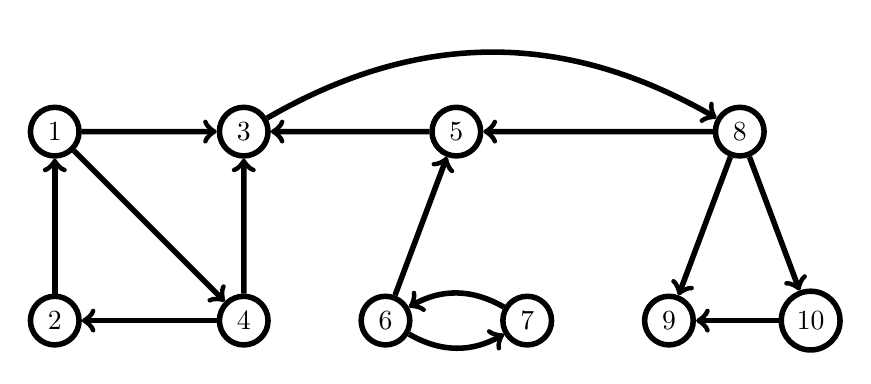
\begin{tikzpicture}[line width=2,scale=1.2]
	 \node[circle,draw=black] (1) at (0,2) {$1$};
	 \node[circle,draw=black] (2) at (0,0) {$2$};
	 \node[circle,draw=black] (3) at (2,2) {$3$};
	 \node[circle,draw=black] (4) at (2,0) {$4$};
	 \node[circle,draw=black] (5) at (4.25,2) {$5$};
	 \node[circle,draw=black] (6) at (3.5,0) {$6$};
	 \node[circle,draw=black] (7) at (5,0) {$7$};
	 \node[circle,draw=black] (8) at (7.25,2) {$8$};
	 \node[circle,draw=black] (9) at (6.5,0) {$9$};
	 \node[circle,draw=black] (10) at (8,0) {$10$};
		
	 \draw[<-] (1) edge (2);
	 \draw[<-] (2) edge (4);
	 \draw[<-] (3) edge (1) (3) edge (4) (3) edge (5);
	 \draw[<-] (4) edge (1);
	 \draw[<-] (5) edge (6) (5) edge (8); 
	 \draw[<-] (6) to[bend left] (7);
	 \draw[<-] (7) to[bend left] (6);
	 \draw[<-] (8) to[bend right] (3);
	 \draw[<-] (9) edge (8) (9) edge (10);
	 \draw[<-] (10) edge (8); 
\end{tikzpicture}
	&
$\leadsto$
	&
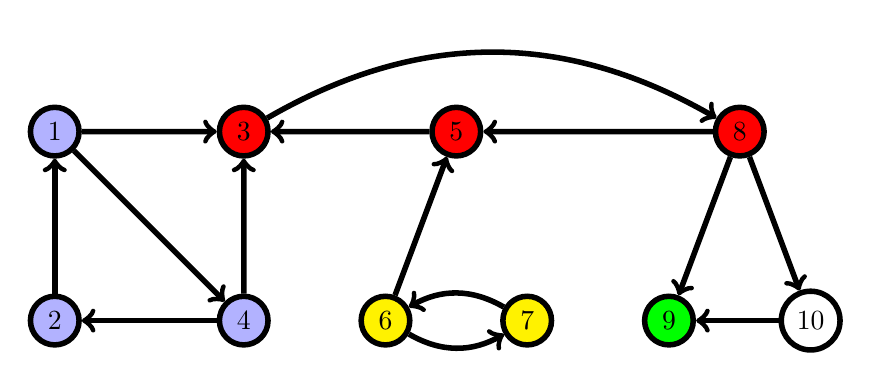
\begin{tikzpicture}[line width=2,scale=1.2]
	\node[fill=blue!30!white,circle,draw] (1) at (0,2) {$1$};
	\node[fill=blue!30!white,circle,draw] (2) at (0,0) {$2$};
	\node[fill=red,circle,draw] (3) at (2,2) {$3$};
	\node[fill=blue!30!white,circle,draw] (4) at (2,0) {$4$};
	\node[fill=red,circle,draw] (5) at (4.25,2) {$5$};
	\node[fill=yellow,circle,draw] (6) at (3.5,0) {$6$};
	\node[fill=yellow,circle,draw] (7) at (5,0) {$7$};
	\node[fill=red,circle,draw] (8) at (7.25,2) {$8$};
	\node[fill=green,circle,draw] (9) at (6.5,0) {$9$};
	\node[circle,draw=black] (10) at (8,0) {$10$};
		
	 \draw[<-] (1) edge (2);
	 \draw[<-] (2) edge (4);
	 \draw[<-] (3) edge (1) (3) edge (4) (3) edge (5);
	 \draw[<-] (4) edge (1);
	 \draw[<-] (5) edge (6) (5) edge (8); 
	 \draw[<-] (6) to[bend left] (7);
	 \draw[<-] (7) to[bend left] (6);
	 \draw[<-] (8) to[bend right] (3);
	 \draw[<-] (9) edge (8) (9) edge (10);
	 \draw[<-] (10) edge (8); 
\end{tikzpicture}	
\end{tabular}
} % end of \centering
\end{bsp}

\begin{defn}
	Der \textbf{Komponentengraph} $D^K=(V^K,A^K)$ eines Digraphen $D=(V,A)$
	ist der Digraph, dessen Knotenmenge $V^K$ der Menge aller SZKn von $D$ entspricht, und für $U,W \in V^K$ die Kante $(U,W) \in A^K$ genau dann existiert, falls es ein $u \in U$ und ein $w \in W$ gibt mit $(u,w) \in A$. 
\end{defn}


\begin{bsp}
	\label{bsp:komponentengraph}
	Die starken Zusammenhangskomponenten des Digraphen aus Beispiel~\ref{bsp:tiefensuche} bestehen aus den Knoten gleicher Farbe in folgender Abbildung:
	
	\hfill
	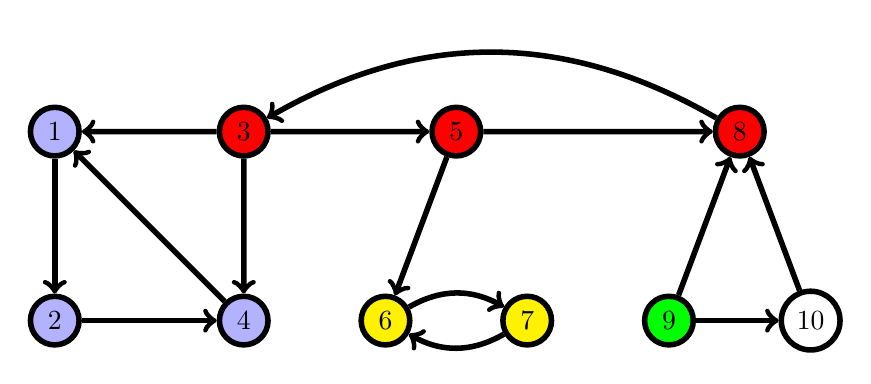
\begin{tikzpicture}[line width=2,scale=1.2]
		\node[fill=blue!30!white,circle,draw] (1) at (0,2) {$1$};
		\node[fill=blue!30!white,circle,draw] (2) at (0,0) {$2$};
		\node[fill=red,circle,draw] (3) at (2,2) {$3$};
		\node[fill=blue!30!white,circle,draw] (4) at (2,0) {$4$};
		\node[fill=red,circle,draw] (5) at (4.25,2) {$5$};
		\node[fill=yellow,circle,draw] (6) at (3.5,0) {$6$};
		\node[fill=yellow,circle,draw] (7) at (5,0) {$7$};
		\node[fill=red,circle,draw] (8) at (7.25,2) {$8$};
		\node[fill=green,circle,draw] (9) at (6.5,0) {$9$};
		\node[circle,draw=black] (10) at (8,0) {$10$};
		
		\draw[->] (1) edge (2);
		\draw[->] (2) edge (4);
		\draw[->] (3) edge (1) (3) edge (4) (3) edge (5);
		\draw[->] (4) edge (1);
		\draw[->] (5) edge (6) (5) edge (8); 
		\draw[->] (6) to[bend left] (7);
		\draw[->] (7) to[bend left] (6);
		\draw[->] (8) to[bend right] (3);
		\draw[->] (9) edge (8) (9) edge (10);
		\draw[->] (10) edge (8); 
	\end{tikzpicture}
	\hfill\,
	
\vspace{1em}
\noindent Der Komponentengraph dieses  Digraphen ist: 
\begin{center} 
	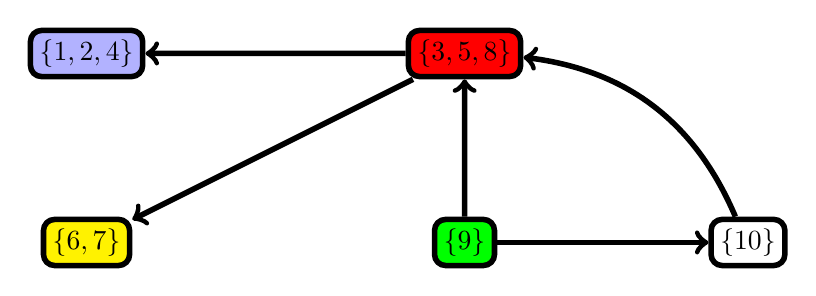
\begin{tikzpicture}[line width=2,scale=1.2]
		\node[fill=blue!30!white,rounded corners,draw] (1) at (2,2) {$\{1,2,4\}$};
		% \node[fill=blue,rounded corners,draw] (2) at (0,0) {$2$};
		% \node[fill=red,rounded corners,draw] (3) at (2,2) {$3$};
		% \node[fill=blue,rounded corners,draw] (4) at (2,0) {$4$};
		\node[fill=red,rounded corners,draw] (5) at (6,2) {$\{3,5,8\}$};
		\node[fill=yellow,rounded corners,draw] (6) at (2,0) {$\{6,7\}$};
		% \node[fill=yellow,rounded corners,draw] (7) at (5,0) {$7$};
		% \node[fill=red,rounded corners,draw] (8) at (7.25,2) {$8$};
		\node[fill=green,rounded corners,draw] (9) at (6,0) {$\{9\}$};
		\node[rounded corners,draw=black] (10) at (9,0) {$\{10\}$};
		
		\draw[->] (5) edge (6) (5) edge (1); 
		\draw[->] (9) edge (5) (9) edge (10);
		\draw[->] (10) to[bend right] (5); 
	\end{tikzpicture}
\end{center}
\end{bsp}


\begin{prop}\label{prop:kompgraph-azyklisch}
	Der Komponentengraph eines jeden Digraphen ist azyklisch. 
\end{prop}
\begin{proof}
Sei $D=(V,A)$ ein Digraph und $D^K$ sein Komponentengraph.
Angenommen, es gibt einen Zyklus in $D^K=(V^K,A^K)$.
Dann gibt es SZKn $K_1,K_2 \in V^K$ mit $K_1 \neq K_2$ und sowohl einen $(K_1,K_2)$-Pfad als auch einen $(K_2,K_1)$-Pfad in $D^K$.
Diese Pfade können jeweils durch weitere SZKn verlaufen.

Das heißt aber, dass für je zwei Knoten $u \in K_1$ und $v \in K_2$ ein $(u,v)$-Pfad und ein $(v,u)$-Pfad in $D$ existiert.
Damit ist dann $K_1 \cup K_2$ stark zusammenhängend, aber Knoten $u \in K_1$ und $v \in K_2$ waren mittels $K_1 \neq K_2$ als nicht äquivalent angenommen.

Dieser Widerspruch zeigt, dass es in $D^K$ keinen Zyklus geben kann.
\end{proof}

\begin{bem}
Wir benötigen noch mehr Verständnis der Beziehungen zwischen den Zeitstempeln, die während der Laufzeit der Tiefensuche auf $D=(V,A)$ erzeugt werden.
Wenn wir nachfolgend von Zeitpunkten der Entdeckung und Abarbeitung sprechen, dann beziehen wir uns stets auf die entsprechenden Zeitstempel der ersten Tiefensuche in Zeile~\ref{line:szhk0} von $\cc{SZK}(D)$.

Für die Formulierung der Aussage erweitern wir zunächst die Begriffe der Entde\-ckungs- und Abarbeitungszeitpunkte von einzelnen Knoten auf Teilmengen von Knoten:

Für $U \subseteq V$ seien dazu
\[
\cc{Grau}(U) := \min_{u \in U} \,\cc{Grau}[u] \quad \text{ und } \quad\cc{Schwarz}(U) := \max_{u \in U} \,\cc{Schwarz}[u]
\]
der früheste Entdeckungszeitpunkt beziehungsweise der späteste Abarbeitungszeitpunkt eines Knotens aus~$U$.
\end{bem}

\begin{lem}
\label{lem:komponenten-zeitpunkte}
Sei $D=(V,A)$ ein Digraph und seien $K,K'$ zwei verschiedene starke Zusammenhangskomponenten von~$D$.
\begin{enuma}
 \item\label{lem:komponenten-zeitpunkte:primal} Falls eine Kante $(u,v) \in A$ mit $u \in K$ und $v \in K'$ existiert, so gilt
 \[
 \cc{Schwarz}(K) > \cc{Schwarz}(K').
 \]
 
 \item\label{lem:komponenten-zeitpunkte:transponiert} Falls eine Kante $(u,v) \in A^\top$ mit $u \in K$ und $v \in K'$ existiert, so gilt
 \[
 \cc{Schwarz}(K) < \cc{Schwarz}(K').
 \]
\end{enuma}
\end{lem}

\condclearpage

\begin{proof}
(a): Wir unterscheiden Fälle danach welche der beiden starken Zusammenhangskomponenten zuerst entdeckt wird.

Sei zuerst angenommen, dass $\cc{Grau}(K) < \cc{Grau}(K')$ gilt und sei~$x$ der erste entdeckte Knoten in~$K$.
Zum Zeitpunkt $\cc{Grau}[x]$ sind alle anderen Knoten in~$K$ und alle Knoten in~$K'$ weiß.
In diesem Moment enthält~$D$ also Pfade von~$x$ zu jedem anderen Knoten in~$K$, die, bis auf~$x$ selbst, nur aus weißen Knoten bestehen.
Die Existenz der Kante $(u,v)$ von der Komponente~$K$ in die Komponente~$K'$ impliziert damit, dass ebenso Pfade von~$x$ zu jedem Knoten in~$K'$ bestehen, die, bis auf~$x$ selbst, nur aus weißen Knoten bestehen.

Nach dem Theorem der weißen Pfade (Korollar~\ref{kor:weisse:pfade}) und dem Klammerungstheorem (Theorem~\ref{thm:klammerung}) werden also alle Knoten in $K \cup K'$ während $\cc{TS}(x)$ entdeckt und sind Nachfahren von~$x$ im Tiefensuchwald.
Nach Korollar~\ref{cor:nachfahre-tiefenwald} erhalten wir damit $\cc{Schwarz}(K) = \cc{Schwarz}[x] > \cc{Schwarz}(K')$.

\condclearpage

Sei nun angenommen, dass $\cc{Grau}(K) > \cc{Grau}(K')$ gilt und sei~$y$ der erste entdeckte Knoten in~$K'$.
Analog zu oben sind zum Zeitpunkt $\cc{Grau}[y]$ alle Knoten in~$K'$ mit einem Pfad von~$y$ aus erreichbar, der, bis auf~$y$ selbst, nur aus weißen Knoten besteht.
Damit sind wieder alle Knoten aus~$K'$ Nachfahren von~$y$ im Tiefensuchwald und mit Korollar~\ref{cor:nachfahre-tiefenwald} gilt $\cc{Schwarz}[y] = \cc{Schwarz}(K')$.

Nach Annahme sind zum Zeitpunkt $\cc{Grau}[y]$ alle Knoten in~$K$ weiß.
Da die Kante $(u,v)$ von~$K$ nach~$K'$ existiert und nach Proposition~\ref{prop:kompgraph-azyklisch} der Komponentengraph von~$D$ azyklisch ist, kann es keinen Pfad von einem Knoten in~$K'$ zu einem Knoten in~$K$ geben.
Da damit kein Knoten in~$K$ von~$y$ aus erreichbar ist, ist die ganze Komponente~$K$ zum Zeitpunkt $\cc{Schwarz}[y]$ noch immer weiß.
Als Konsequenz erhalten wir $\cc{Schwarz}[w] > \cc{Schwarz}[y]$, für jeden Knoten $w \in K$, und damit $\cc{Schwarz}(K) > \cc{Schwarz}(K')$.

\condclearpage

(b): Nach der Definition des transponierten Graphen folgt aus der Existenz einer Kante $(u,v) \in A^\top$, die Existenz der Kante $(v,u)$ in~$D$.
Nach Teil (a) gilt damit $\cc{Schwarz}(K') > \cc{Schwarz}(K)$.
\end{proof}

\begin{bem}
\underline{Grundidee des Korrektheitsbeweises von $\cc{SZK}(D)$:}
\begin{itemize}
 \item Die Tiefenssuche auf~$D^\top$ startet in der starken Zusammenhangskomponente~$K_1$, die den zuletzt abgearbeiteten Knoten~$u_1$ der Tiefensuche auf~$D$ enthält.
 \item Der transponierte Graph $D^\top$ enthält nach Lemma~\ref{lem:komponenten-zeitpunkte}~\ref{lem:komponenten-zeitpunkte:transponiert} keine Kanten, die von~$K_1$ zu einer anderen starken Zusammenhangskomponente verlaufen.
 \item Die Tiefensuche in $D^\top$, die von~$u_1$ aus startet besucht also genau die Knoten aus der Komponente~$K_1$.
 \item Der Algorithmus wählt danach den Knoten~$u_2$ außerhalb der Komponente~$K_1$, der als letztes unter den verbleibenden Knoten bei der Tiefensuche auf~$D$ abgearbeitet wurde und besucht wie zuvor, alle Knoten der starken Zusammenhangskomponente~$K_2$, die~$u_2$ enthält.
 \item Dies geht iterativ weiter bis alle Tiefensuchbäume erstellt sind, und wir sehen, dass diese den starken Zusammenhangskomponenten entsprechen.
\end{itemize}
\end{bem}


\begin{thm}
Der Algorithmus $\cc{SZK}(D)$ bestimmt die starken Zusammenhangskomponenten eines Digraphen $D=(V,A)$ korrekt.
\end{thm}
\begin{proof}
Wir argumentieren mittels vollständiger Induktion nach der Anzahl $k$ der Tiefensuch\-bäume, die bei der Tiefensuche auf $D^\top$ in den Zeilen~\ref{line:szhk1}-\ref{line:szhk2} des Algorithmus $\cc{SZK}(D)$ gefunden werden und zeigen, dass jeder solche Baum eine starke Zusammenhangskomponente bildet.
Die konkrete Aussage, die wir per Induktion beweisen, ist:
\begin{center}
\glqq Die ersten $k$ Tiefensuchbäume, die in den Zeilen~\ref{line:szhk1}-\ref{line:szhk2} erzeugt werden, sind starke Zusammenhangskomponenten von~$D$.\grqq
\end{center}

\noindent Der Induktionsanfang ist mit $k=0$ klar.
Für den Induktionsschritt, sei $B \subseteq V$ der $(k+1)$-te erzeugte Baum bei der Tiefensuche auf~$D^\top$.
Sei weiterhin $u \in B$ die Wurzel dieses Baumes und $K \subseteq V$ die starke Zusammenhangskomponente, die~$u$ enthält.
Für jede starke Zusammenhangskomponente $K' \neq K$, die bereits besucht wurde, gilt $\cc{Schwarz}[u] = \cc{Schwarz}(K) < \cc{Schwarz}(K')$, wegen der Reihenfolge in der die Knoten in Zeile~\ref{line:szhk2} durchlaufen werden.
Wegen der Induktionsannahme sind zum Zeitpunkt zu dem die Suche den Knoten~$u$ besucht, alle anderen Knoten von~$K$ weiß.
Wie zuvor sind nach dem Theorem der weißen Pfade und dem Klammerungstheorem daher alle anderen Knoten in~$K$ Nachfahren von~$u$ in dessen Tiefensuchbaum~$B$.

Weiterhin müssen nach Induktionsannahme und Lemma~\ref{lem:komponenten-zeitpunkte}~\ref{lem:komponenten-zeitpunkte:transponiert} alle Kanten von~$D^\top$, die aus $K$ herausführen, zu starken Zusammenhangskomponenten verlaufen, die bereits entdeckt wurden.
Damit wird kein Knoten außerhalb von~$K$ ein Nachfahre von~$u$ bei der Tiefensuche auf~$D^\top$.
Das heißt, dass die Knoten des Tiefensuchbaumes von~$D^\top$, der von~$u$ ausgeht, eine starke Zusammenhangskomponente bilden, und der Induktionsschritt ist gezeigt.
\end{proof}


\begin{bem}
	Die Präsentation der Tiefensuche basiert auf  \cite{CLRS17}.
\end{bem} 